%---------------------------------------------------------
%\VideoClassification[column=3,colour=blue,nodev, nodevops,nobus]
%\VideoClassification[column=3,colour=blue,nodev, nodevops,nobus]
%\VideoClassification[nodev, column=2]

%\VideoClassification[column=3, colour=blue]
%
%%---------------------------------------------------------
%
%
%\section{Introduction To Data Management and Data Warehouse}
%
%%%%%%%%%%%%%%%%%%%%%%%%%%%%%%%%%%%%%%%%%%%%%%%%%%%%%%%%%%%%%%%%%%%%%%%%%%%%%%%%%%%%%%%%%%
%
%\begin{frame}
%\frametitle{Chapter Objectives}
%
%\begin{itemize}[<+->]
%	\item Be familiar with data management life-cycle.
%	\item Understand the data abstraction and the data layer.
%	\item Motivation to DWH.
%	\item What are the different types of DWH?
%	\item Usecases for DWH. How is it different from the operational DB?
%	\item Explain the data Encoding and Formats.
%	\item Show what the challenges of building a DWH are?
%	\item What are the data modeling and its design?
%\end{itemize}
%%https://opentextbc.ca/dbdesign01/chapter/chapter-5-data-modelling/
%\end{frame}
%
%%%%%%%%%%%%%%%%%%%%%%%%%%%%%%%%%%%%
%
%\subsection{Data Management}
%
%\begin{frame}
%\frametitle{Data Management}
%
%\begin{itemize}[<+->]
%\item Data are a product.
%\item Data product has a life-cycle as following (simplified):
%\begin{itemize}[<+->]
%	\item \textbf{Question}, Idea, or service.
%	\item \textbf{Identify} the source of information and the data type.
%	\item \textbf{Document} all details regarding the data including quality, security, efficiency, and access (consideration during the cycle).
%	\item Delivery automation (Tools and Process). AKA \textbf{DevOps} cycle.
%	\item Data Architecture (model design and rules).
%	\item \textbf{Extraction}, \textbf{Transformation}, and \textbf{Loading} Process.
%	\item Business Intelligence (\textbf{BI}) or data discovery (continues process).
%	\item \textbf{Integration} and publishing.
%	\item Data retention or \textbf{archiving} process \forexample (Hot or Cold storage).
%\end{itemize}
%\end{itemize}
%
%\end{frame}
%
%%%%%%%%%%%%%%%%%%%%%%%%%%%%%%%%%%%%%%%%%%%%%%%%%%%%%%%%%%%%%%%%%%%%%%%%%%%%%%%%%%%%%%%%%%
%
%\begin{frame}
%\frametitle{Data Management Life-Cycle}
%\scalebox{0.9}{
%
%\smartdiagramset{circular distance=3.5cm,
%font=\scriptsize,
%%				text width=1cm,
%module minimum width=2cm,
%circular distance =3.4cm,
%module minimum height=.1cm,
%arrow tip=to}
%\smartdiagram[circular diagram]{Archiving,Idea, Identify, Document, 				
%DevOps, Arch.,ETL, BI, Integration}
%}
%\end{frame}
%
%%---------------------------------------------------------
%\VideoClassification[column=2, colour=blue]
%%%%%%%%%%%%%%%%%%%%%%%%%%%%%%%%%%%%%%%%%%%%%%%%%%%%%%%
%\subsection{Data Abstraction}
%\begin{frame}
%	\frametitle{Motivation to Data Layers (Use Case)}	
%	    \begin{figure}[H]
    	\smartdiagramset{
    		%descriptive items y sep = 3em,
    		description font = \scriptsize\sffamily,
    		description title font=\scriptsize\sffamily,
    	}
%	\centering
	\begin{subfigure}[t]{0.475\textwidth}
%		\centering
		\scalebox{0.5}{
		\smartdiagram[descriptive diagram]{
			{App, Application UI},
			{FS, CSV Data}}
		}
		\vspace{-.6\baselineskip}
		\caption{{\tiny Two layers Arch. (Data \& UI)}}
		\label{fig:ch_1_data_abstraction_1}
	\end{subfigure}
	\hfill
	\begin{subfigure}[t]{0.475\textwidth}
%		\centering 
		\scalebox{0.5}{
			\smartdiagram[descriptive diagram]{
				{App, Application UI},
				{BL, CSV Data Loader (Reporting)},
				{FS, CSV Data}}
			}
		\vspace{-.6\baselineskip}
		\caption{{\tiny Three layers Arch. (Data \& BL \& UI)}}
		\label{fig:ch_1_data_abstraction_2}
	\end{subfigure}
%	\vskip\baselineskip
	\begin{subfigure}[t]{0.475\textwidth}   
%		\centering 
		\scalebox{0.5}
		{
			\smartdiagram[descriptive diagram]{
			{App, Application UI},
			{BL, (JSON/CSV) Data Loader (Reporting)},
			{FS, JSON Data}}
		}
		\vspace{-.6\baselineskip}
		\caption{{\tiny Three layers Arch. (Data (multi-sources) \& BL \& UI)}}
		\label{fig:ch_1_data_abstraction_3}
	\end{subfigure}
	\quad
	\begin{subfigure}[t]{0.475\textwidth}   
%		\centering 
		\scalebox{0.5}
		{
			\smartdiagram[descriptive diagram]{
				{App, Application UI},
				{DBMS-H, Ready prepared layer for each department (Reporting)},
				{DBMS-M, Logical part to prepare for the data structure and the relation between the data},
				{DBMS-L, Storage and Data format related stuff + Data indexing and searching algorithms}}
		}
		\vspace{-.6\baselineskip}
		\caption{{\tiny Four layers Arch. (DB (L, M, H) \& UI)}}
		\label{fig:ch_1_data_abstraction_4}
	\end{subfigure}
	\vspace{-.6\baselineskip}
	\caption {\tiny Data Abstraction Journey} 
	\label{fig:ch_1_data_abstraction}
	\end{figure}
	
	
%
%\end{frame}
%%%%%%%%%%%%%%%%%%%%%%%%%%%%%%%%%%%%%%%%%%%%%%%%%%%%%%%
%\begin{frame}
%	\frametitle{Motivation to Data Layers (Solution Thinking)}
%	
%	\begin{itemize}[<+->]
%		\item How can we think about a data solution or challenges in the data products?
%		\begin{itemize}[<+->]
%			\item Requirements analysis.
%			\item Identify the problem (challenges).
%			\item Think about how to overcome the challenges.
%			\item Ask your self the following questions:
%			\begin{itemize}[<+->]
%				\item Can we solve the problem using the current data structure by adding new features?
%				\item What if we enhance/change the data structure or modeling?
%				\item Could it help if we change the backend engine \forexample (DBMS system)?
%			\end{itemize}			
%		\end{itemize}
%		\item To answer these questions you need to understand the \textbf{\underline{data layers}}.
%	\end{itemize}
%	
%\end{frame}
%%%%%%%%%%%%%%%%%%%%%%%%%%%%%%%%%%%%%%%%%%%%%%%%%%%%%%%
%\begin{frame}
%	\frametitle{Data Layers (Abstraction)}
%	\begin{itemize}[<+->]
%		\item Any data product (database) contains multi-layers.
%		\item Each layer responsible for different tasks and operations.
%		\item Each layer interacts with (hardware or software or mixed).
%		\item Eliminate the complexity of data interactions; not all internal processes are shared or available for the user.
%		\item The developer for each layer hides irrelevant internal details from the developer (users). 
%		\item The process of \textbf{\underline{\blue{hiding}}} irrelevant details from the developer (user) is called data \textbf{\underline{\blue{abstraction}}}.
%	\end{itemize}	
%\end{frame}
%%%%%%%%%%%%%%%%%%%%%%%%%%%%%%%%%%%%%%%%%%%%%%%%%%%%%%%
%\begin{frame}
%	\frametitle{Data Layers (Abstraction)}
%	\begin{definition}
%		\textbf{Data Abstraction and Data Independence}: DBMS comprises complex data-structures. To make the system efficient in terms of retrieval of data and reduce complexity in terms of usability of users, developers use abstraction i.e., hide irrelevant details from the users. This approach simplifies database design.
%		%https://www.geeksforgeeks.org/data-abstraction-and-data-independence/
%	\end{definition}	
%	%Capacity of changing in one level without affecting the other levels. Copied but forget from where!!!
%	\begin{itemize}[<+->]
%		\item There are 3 levels of data abstraction.
%		\begin{itemize}[<+->]
%			\item Physical Level
%			\item Logical/Conceptual Level.
%			\item View Level.
%		\end{itemize}
%	\end{itemize}	
%	%TOP TIER, MIDDLE TIER, BOTTOM TIER
%\end{frame}
%%%%%%%%%%%%%%%%%%%%%%%%%%%%%%%%%%%%%%%%%%%%%%%%%%%%%%%
%\begin{frame}
%\frametitle{Data Layers (Abstraction)}
%	\scalebox{0.9}{
\begin{tikzpicture}[node distance=2cm,
					every node/.style={fill=white, font=\sffamily}, align=center,
					scale=0.6, 
					every node/.style={transform shape}]

% Specification of nodes (position, etc.)
\node (view2)             [optionalETL]              {report 2 (view)};
\node (view1)     [optionalETL, right of=view2, xshift=3cm]          {report 1 (view)};
\node (view3)      [optionalETL, right of=view1, xshift=3cm]   {report 3 (view)};
\node (concept)     [required,below of=view1, yshift=-1.5cm]   {Conceptual Layer};
\node (physical)      [optionalELK, below of=concept, yshift=-1.5cm] {Physical Interaction};
\node (fs)      [optionalELK, below of=physical, yshift=-1cm] {FS};

%\node (Appendix) [startstop, above of=Arch] {Ch.13 Appendix};     
% Normal Path
\draw[<->]     (view2) -- (concept);
\draw[<->]     (view3) -- (concept);
\draw[<->]     (view1) -- (concept);
\draw[<->]     (concept) -- (physical);
\draw[<->]     (fs) -- (physical);
\draw[-]      (12,-1.5) to[out=0,in=180] (13,0)  node[right]{View Level (User View) } to[out=180,in=0] (12,1.5);
\draw[-]      (12,-5) to[out=0,in=180] (13,-3.5) node[right]{Logical/ Conceptual Level } to[out=180,in=0]  (12,-2);
\draw[-]      (12,-11) to[out=0,in=180] (13,-8.5) node[right]{Physical Level } to[out=180,in=0]  (12,-6);
\end{tikzpicture}
}
%\end{frame}
%%---------------------------------------------------------
%\VideoClassification
%%%%%%%%%%%%%%%%%%%%%%%%%%%%%%%%%%%%%%%%%%%%%%%%%%%%%%%
%\begin{frame}
%	\frametitle{Physical level}
%	\begin{itemize}[<+->]
%		\item \textbf{Physical level (Internal)}: 
%		\begin{itemize}[<+->]
%			\item Lowest level.
%			\item Describes \textbf{\underline{\blue{how}}} data is stored.
%			\item Describes the data structure.
%			\item It allows you to modify the lowest level (Physical part) without any change in the logical schema. These change could be
%				\begin{itemize}[<+->]				
%					\item Using a new storage device
%					\item Change the structure of the data used for storage
%					\item Change the file type or use a different storage structure
%					\item Chang the access method
%					\item Modify indexes
%					\item Change the compression algorithm or hashing technique.
%			\end{itemize}									
%		\end{itemize}		
%		%https://beginnersbook.com/2015/04/levels-of-abstraction-in-dbms/		
%		%https://www.guru99.com/dbms-data-independence.html
%	\end{itemize}	
%\end{frame}
%%%%%%%%%%%%%%%%%%%%%%%%%%%%%%%%%%%%%%%%%%%%%%%%%%%%%%%
%\begin{frame}
%	\frametitle{Physical level}
%	\begin{example}		
%		\begin{itemize}[<+->]
%			\item Database contains product information.
%			\item Physical layer describes
%			\begin{itemize}[<+->]
%				\item Storage mechanism and the blocks (bytes, gigabytes, terabytes, etc.).
%				\item The amount of memory used.
%				\item Usually this layer abstracted from the programmers.
%			\end{itemize}
%		\end{itemize}
%	\end{example}
%	
%\end{frame}
%%---------------------------------------------------------
%%---------------------------------------------------------
%\VideoClassification
%%%%%%%%%%%%%%%%%%%%%%%%%%%%%%%%%%%%%%%%%%%%%%%%%%%%%%%
%\begin{frame}
%	\frametitle{Logical level}
%	\begin{itemize}[<+->]
%		\item \textbf{Logical level (Conceptual)}: 
%		\begin{itemize}[<+->]
%			\item Intermediate level
%			\item Describes \textbf{\underline{\blue{what}}} data is stored
%			\item Describes what the relationship between the stored data is?
%			\item It allows you to change the logical view without altering the external view, API, or programs. These change could be
%			\begin{itemize}[<+->]
%				\item Add a new table
%				\item Change the records merge or delete without affecting the running applications
%				\item Change attribute (Add,delete) to the existing table
%			\end{itemize}									
%		\end{itemize}		
%	\end{itemize}	 
%\end{frame}
%%%%%%%%%%%%%%%%%%%%%%%%%%%%%%%%%%%%%%%%%%%%%%%%%%%%%%%
%\begin{frame}
%	\frametitle{Logical level}
%	\begin{example}
%		\begin{itemize}[<+->]
%			\item Database contains product information.
%			\item Logical Layer describes
%			\begin{itemize}[<+->]
%				\item The product fields and their data types
%				\item How this product interact with other entities in the database
%				\item The programmers' design this level based on business knowledge and the requirements
%			\end{itemize}
%		\end{itemize}
%	\end{example}
%	
%\end{frame}
%
%
%%---------------------------------------------------------
%%---------------------------------------------------------
%\VideoClassification
%%%%%%%%%%%%%%%%%%%%%%%%%%%%%%%%%%%%%%%%%%%%%%%%%%%%%%%
%\begin{frame}
%	\frametitle{View level}
%	\begin{itemize}[<+->]
%		\item \textbf{View level (External)}: 
%		\begin{itemize}[<+->]
%			\item Highest level.
%			\item \textbf{\underline{\blue{View}}} of the data stored? 
%			\item Designed for a category of users
%			\item The final interface for the user
%			\item Extended or hidden based on the user's role
%			\item Not all the views is extended to all users, and there is authentication based on the category
%		\end{itemize}		
%	\end{itemize}	
%	
%\end{frame}
%%%%%%%%%%%%%%%%%%%%%%%%%%%%%%%%%%%%%%%%%%%%%%%%%%%%%%%
%\begin{frame}
%	\frametitle{View level}
%	\begin{example}
%		\begin{itemize}[<+->]
%			\item The database contains product information
%			\item It could be designed to show the sales of the product in a specific region
%			\item We might hide information about some products based on the teams or users
%		\end{itemize}
%	\end{example}
%	
%\end{frame}
%
%%---------------------------------------------------------
%%---------------------------------------------------------
%\VideoClassification[column=2, colour=blue]
%%%%%%%%%%%%%%%%%%%%%%%%%%%%%%%%%%%%%%%%%%%%%%%%%%%%%%%
%\begin{frame}[c]
%	\frametitle{Data solution thinking (Summary) }
%	% !!!!!!!!!!!!!! We need to mention that this slide is just an overview there will be a detailed one later
%        \begin{center}
%			Let's answer our previous question. How can we solve data challenges?
%        \end{center}
%    \end{frame}
%
%%%%%%%%%%%%%%%%%%%%%%%%%%%%%%%%%%%%%%%%%%%%%%%%%%%%%%%
%
%%%%%%%%%%%%%%%%%%%%%%%%%%%%%%%%%%%%%%%%%%%%%%%%%%%%%%% 
%\begin{frame}
%	\frametitle{Data solution thinking (Summary) }
%	\begin{itemize}[<+->]
%        \item Let's split the problem based on the data layers.
%          \begin{itemize}[<+->]
%          \item View layer
%            \begin{itemize}[<+->]
%            \item When we need to add/remove/create new reports, it is usually a view layer.
%            \item We don't need to change the logical or physical layer to support the view layer.
%          \end{itemize}
%        \end{itemize}
%       \end{itemize}
% \end{frame}
%
%%%%%%%%%%%%%%%%%%%%%%%%%%%%%%%%%%%%%%%%%%%%%%%%%%%%%%% 
%\begin{frame}
%\frametitle{Data solution thinking (Summary) }
%	\begin{itemize}[<+->]
%        \item Let's split the problem based on the data layers.
%          \begin{itemize}[<+->]
%           \item Logical Layer
%           \begin{itemize}[<+->]
%             \item When you have missing sources into your logical layer, and you need to add this source and its structure.
%             \item There is a performance issue in the existing reports, and you need to change the model. \forexample reduce the join by creating a new join table (\textit{materialized view}).
%             \item Update the data type or the existing relation, which could help to fix some data or performance issues.
%            \end{itemize}
%           \end{itemize}
%        \end{itemize}
% \end{frame}
%
% %%%%%%%%%%%%%%%%%%%%%%%%%%%%%%%%%%%%%%%%%%%%%%%%%%%%%%%
% %%%%%%%%%%%%%%%%%%%%%%%%%%%%%%%%%%%%%%%%%%%%%%%%%%%%%% 
%\begin{frame}
%  \frametitle{Data solution thinking (Summary) }
%  \begin{itemize}[<+->]
%  \item Let's split the problem based on the data layers.
%    \begin{itemize}[<+->]
%    \item Physical Layer
%      \begin{itemize}[<+->]
%      \item When our problem is hard or impossible to fix by optimizing the query (view)/ logical layer, it is time for physical change.
%      \item If we need to change your storage/compression/structure/access technique.
%      \item If we need to change the data orientation structure from row to column or key-value storage, It is time to change the physical layer.
%      \end{itemize}
%    \end{itemize}
%  \end{itemize}
% \end{frame}
%%---------------------------------------------------------
%\VideoClassification[column=2, colour=blue]
%%%%%%%%%%%%%%%%%%%%%%%%%%%%%%%%%%%%%%%%%%%%%%%%%%%%%%%%
%\subsection{Introduction to DWH}
%
%\subsubsection{Motivation to the Data Warehouse (DWH)}
%\begin{frame}
%\frametitle{Motivation to the Data Warehouse (DWH)}
%	\begin{itemize}[<+->]
%		\item Data could be a product for some companies.
%		\item It could be decision support for other products or businesses.
%		\item It could be reporting the results after passing the data life-cycle from storage (Database).
%		\item Some challenges are facing the people who work on data management backend:
%			\begin{itemize}[<+->]
%				\item Performance,
%				\item Integration,
%				\item and Applying analytical functions. %Moving average
%			\end{itemize}
%		\item Vendors who are working on solving the above challenges are creating their product of DWH. Their ultimate goal is to optimize the above points.
%	\end{itemize}
%\end{frame}
%%%%%%%%%%%%%%%%%%%%%%%%%%%%%%%%%%%%%%%%%%%%%%%%%%%%%%%
%\begin{frame}[c]
%\frametitle{Motivation to the Data Warehouse (DWH)}
%
%\begin{definition}[What is Data Warehousing?] A DWH is a technique for collecting and managing data from varied sources to \textbf{provide meaningful business insights}. It is a blend of technologies and components which aids the strategic use of data.%\footnotemark
%\end{definition}
%
%%REF
%Inmon Bill gave the real concept. He is considered the father of the DWH. He had written about a variety of topics for building, usage, and maintenance of the warehouse \& the Corporate Information Factory
%
%%\footnotetext{The definition mentioned in this slides copied from  \href{https://www.guru99.com/data-warehousing.html\#2}{guru99.com} }
%
%\end{frame}
%
%%%%%%%%%%%%%%%%%%%%%%%%%%%%%%%%%%%%%%%%%%%%%%%%%%%%%%%
%
%%%%%%%%%%%%%%%%%%%%%%%%%%%%%%%%%%%%%%%%%%%%%%%%%%%%%%%
%\begin{frame}
%\frametitle{Motivation to the Data Warehouse (DWH)}
%
%\begin{itemize}[<+->]
%	\item The DWH is not a product but an environment.
%	\item It is a process of transforming data into information and make it available to users in a \textbf{timely manner} to make a difference.
%	\item It is an architectural construct of an information system that provides users with current and historical decision support information which is difficult to access or present in the traditional operational data store.
%	\item The DWH is the core of the BI system built for data analysis and reporting.
%\end{itemize}
%
%\end{frame}
%
%%%%%%%%%%%%%%%%%%%%%%%%%%%%%%%%%%%%%%%%%%%%%%%%%%%%%%%
%
%\begin{frame}
%\frametitle{Motivation to the Data Warehouse}
%
%Other names for the Data warehouse system:
%
%\begin{wideitemize}
%\item Decision Support System (DSS).
%\item Business Intelligence Solution.
%\item Executive Information System.
%\item Management Information System.
%\item Analytic Application.
%\item Data Warehouse.
%
%\end{wideitemize}
%
%
%\end{frame}
%
%%---------------------------------------------------------
%\VideoClassification[column=2]
%%%%%%%%%%%%%%%%%%%%%%%%%%%%%%%%%%%%%%%%%%%%%%%%%%%%%%%
%\subsubsection{Differences Between DWH and Operational DB}
%\begin{frame}
%	\frametitle{DWH vs Operational databases}
%	
%	
%	\begin{table}[t]
%		\centering	
%		\resizebox{\columnwidth}{!}{%
%			
%			%		\centering
%			\begin{tabular}{|c | c | c|}
%				\hline
%				\textbf{Metric}  & \textbf{Transactions DB}& \textbf{DWH} \\
%				\hline
%				Volume & GB/TB & TB/PB \\
%				Historical  & Short-term & Long-Term\\
%				rows & <1000M &  1000M>\\
%				Orientation & Product & Subject or multi products\\
%				Business Units & Product team & Multi organizational units\\
%				Normalization & Normalized %due to storage and performance limitation and its design
%				&  Not required (De-normalized in many use cases)\\
%				Data Model & Relational & Star Schema or Multi-dim\\
%				Intelligence&Reporting & Advanced reporting and Machine Learning\\
%				Use cases& Online transactions \& operations & Centeralized storage (360\textdegree)\\
%				\hline
%			\end{tabular}
%			%		\caption{Data Representation Combination Matrix}\label{Tab:Data_Representation_Matrix}
%		}
%	\end{table}
%\end{frame}
%
%%---------------------------------------------------------
%\VideoClassification[column=2, colour=blue]
%%%%%%%%%%%%%%%%%%%%%%%%%%%%%%%%%%%%%%%%%%%%%%%%%%%%%%%
%
%\begin{frame}
%\frametitle{Transactional DB Use cases}
%\begin{figure}[ht]
%	
%	\centering
%	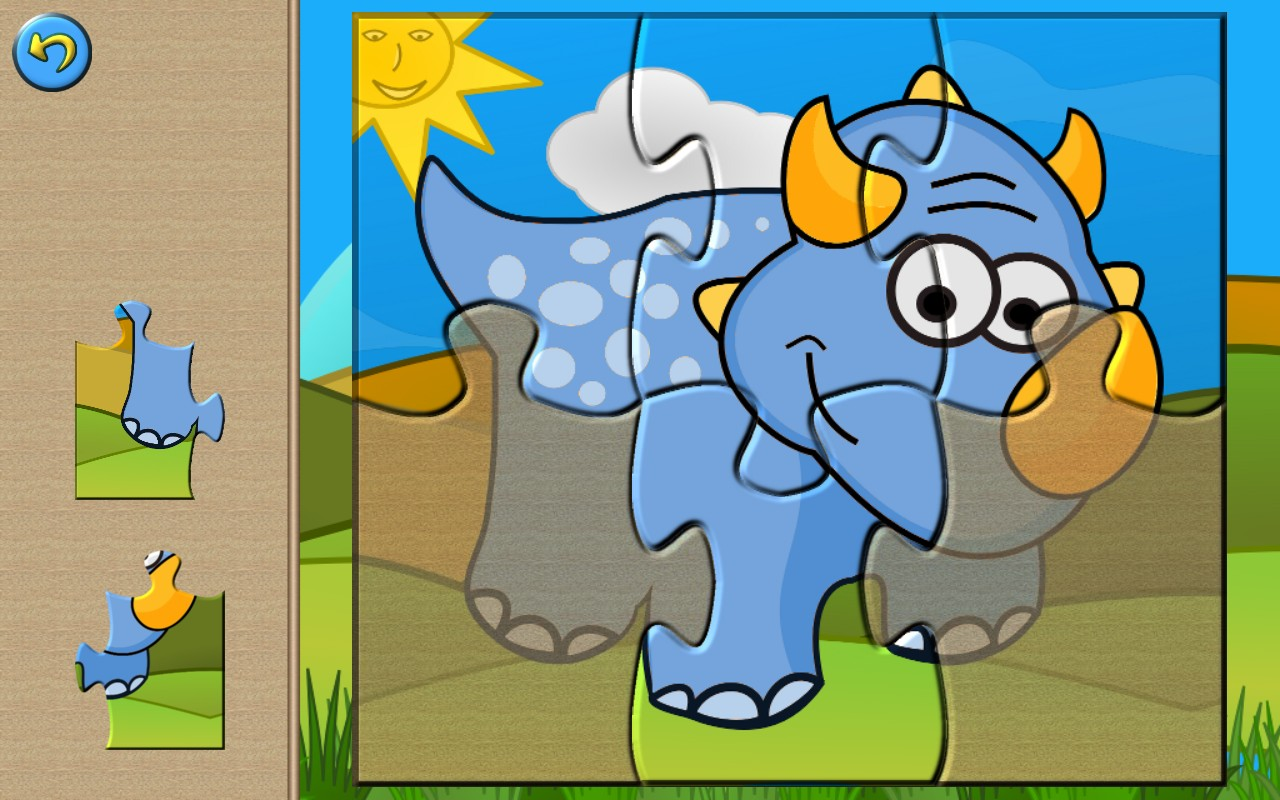
\includegraphics[width=\linewidth]{./Figures/chapter-01/baby-01.jpg}
%	%		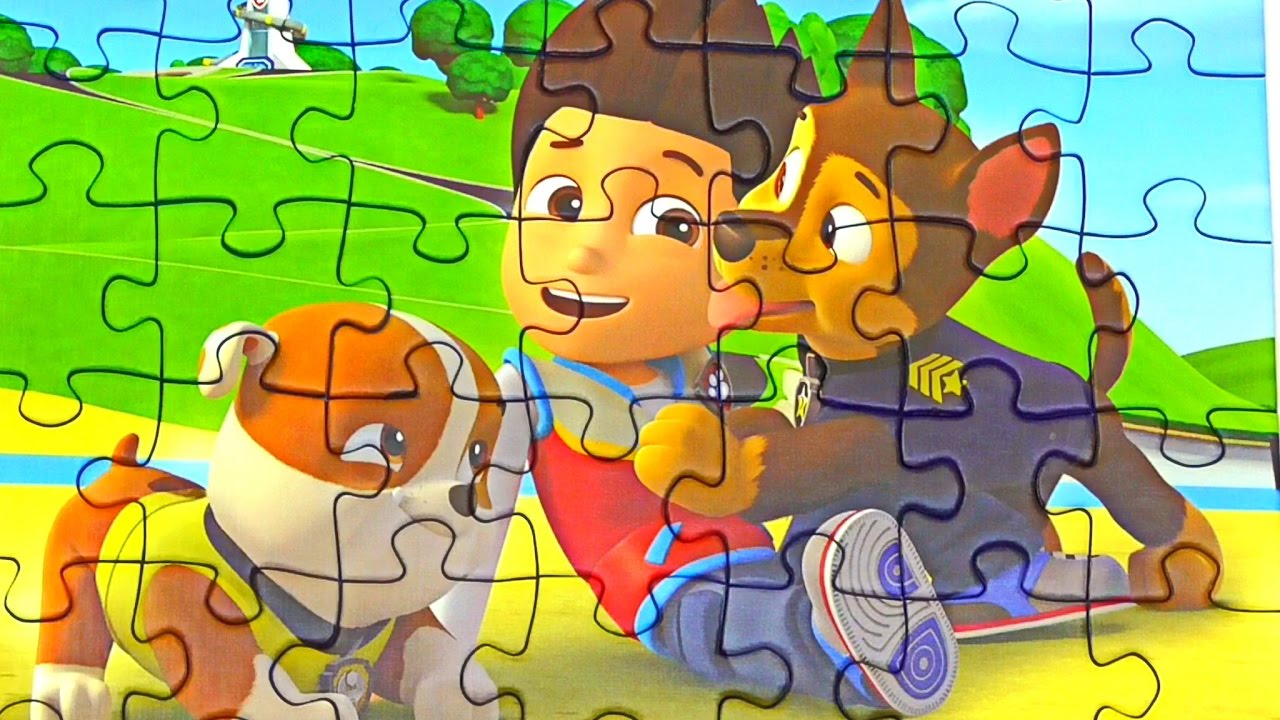
\includegraphics[width=\linewidth,height=\textheight]{./Figures/chapter-01/baby-02.jpg}
%	%	\caption{}
%\end{figure}
%\end{frame}
%
%
%%%%%%%%%%%%%%%%%%%%%%%%%%%%%%%%%%%%%%%%%%%%%%%%%%%%%%%
%\begin{frame}
%\frametitle{Transactional DB Use cases}
%\begin{figure}[ht]
%
%\centering
%%	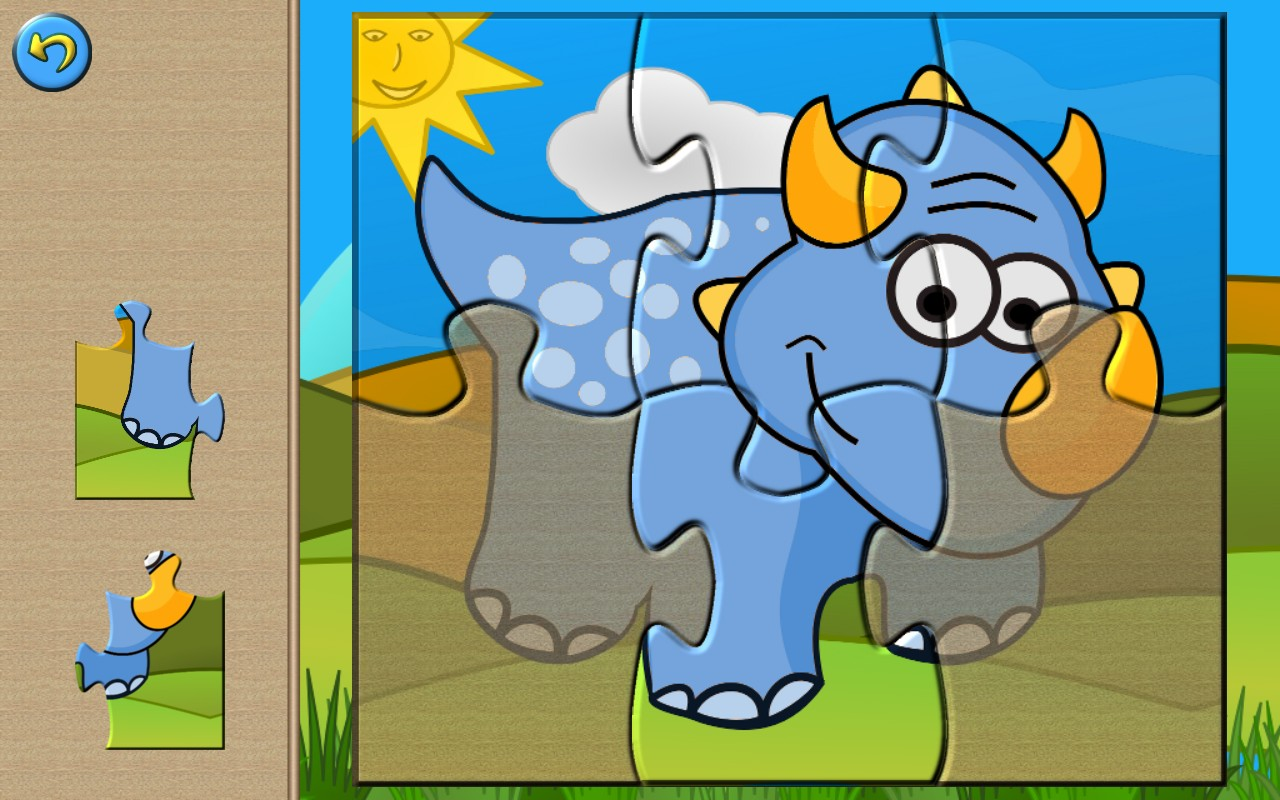
\includegraphics[width=\linewidth]{./Figures/chapter-01/baby-01.jpg}
%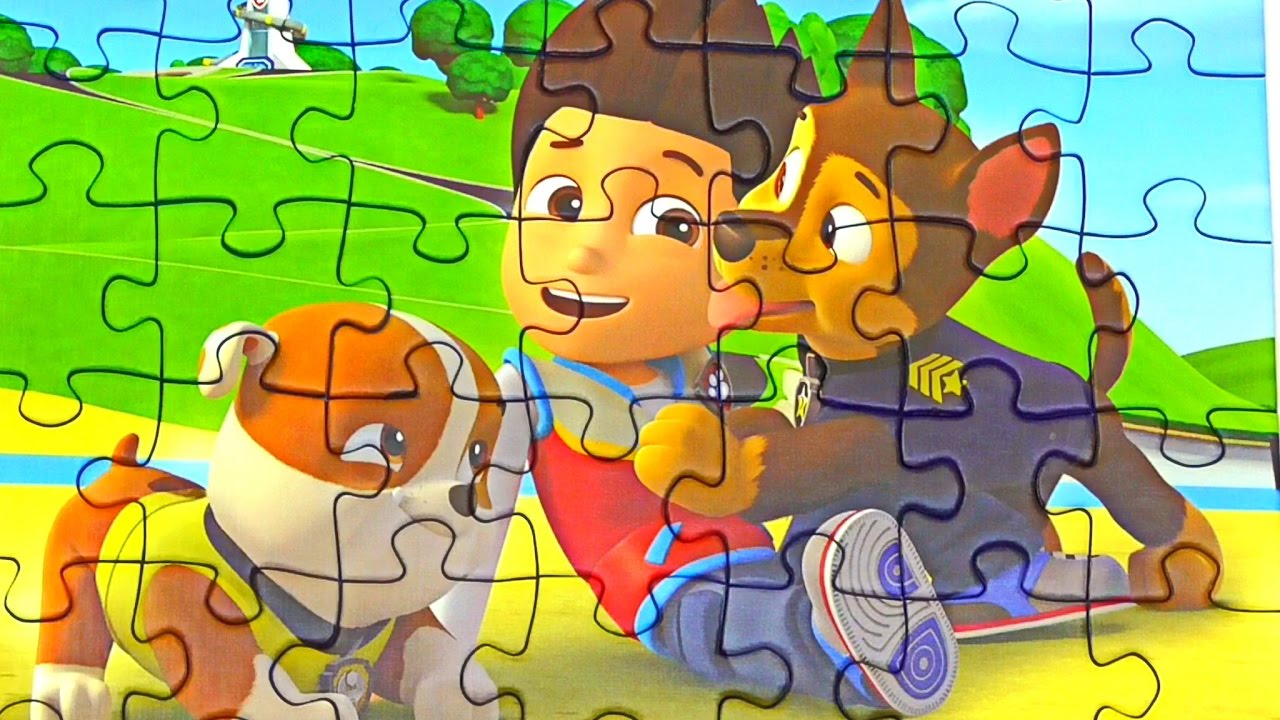
\includegraphics[width=\linewidth]{./Figures/chapter-01/baby-02.jpg}
%%	\caption{}
%\end{figure}
%\end{frame}
%
%
%%%%%%%%%%%%%%%%%%%%%%%%%%%%%%%%%%%%%%%%%%%%%%%%%%%%%%%
%\begin{frame}
%\frametitle{DWH Use cases}
%\begin{figure}[ht]
%
%\centering
%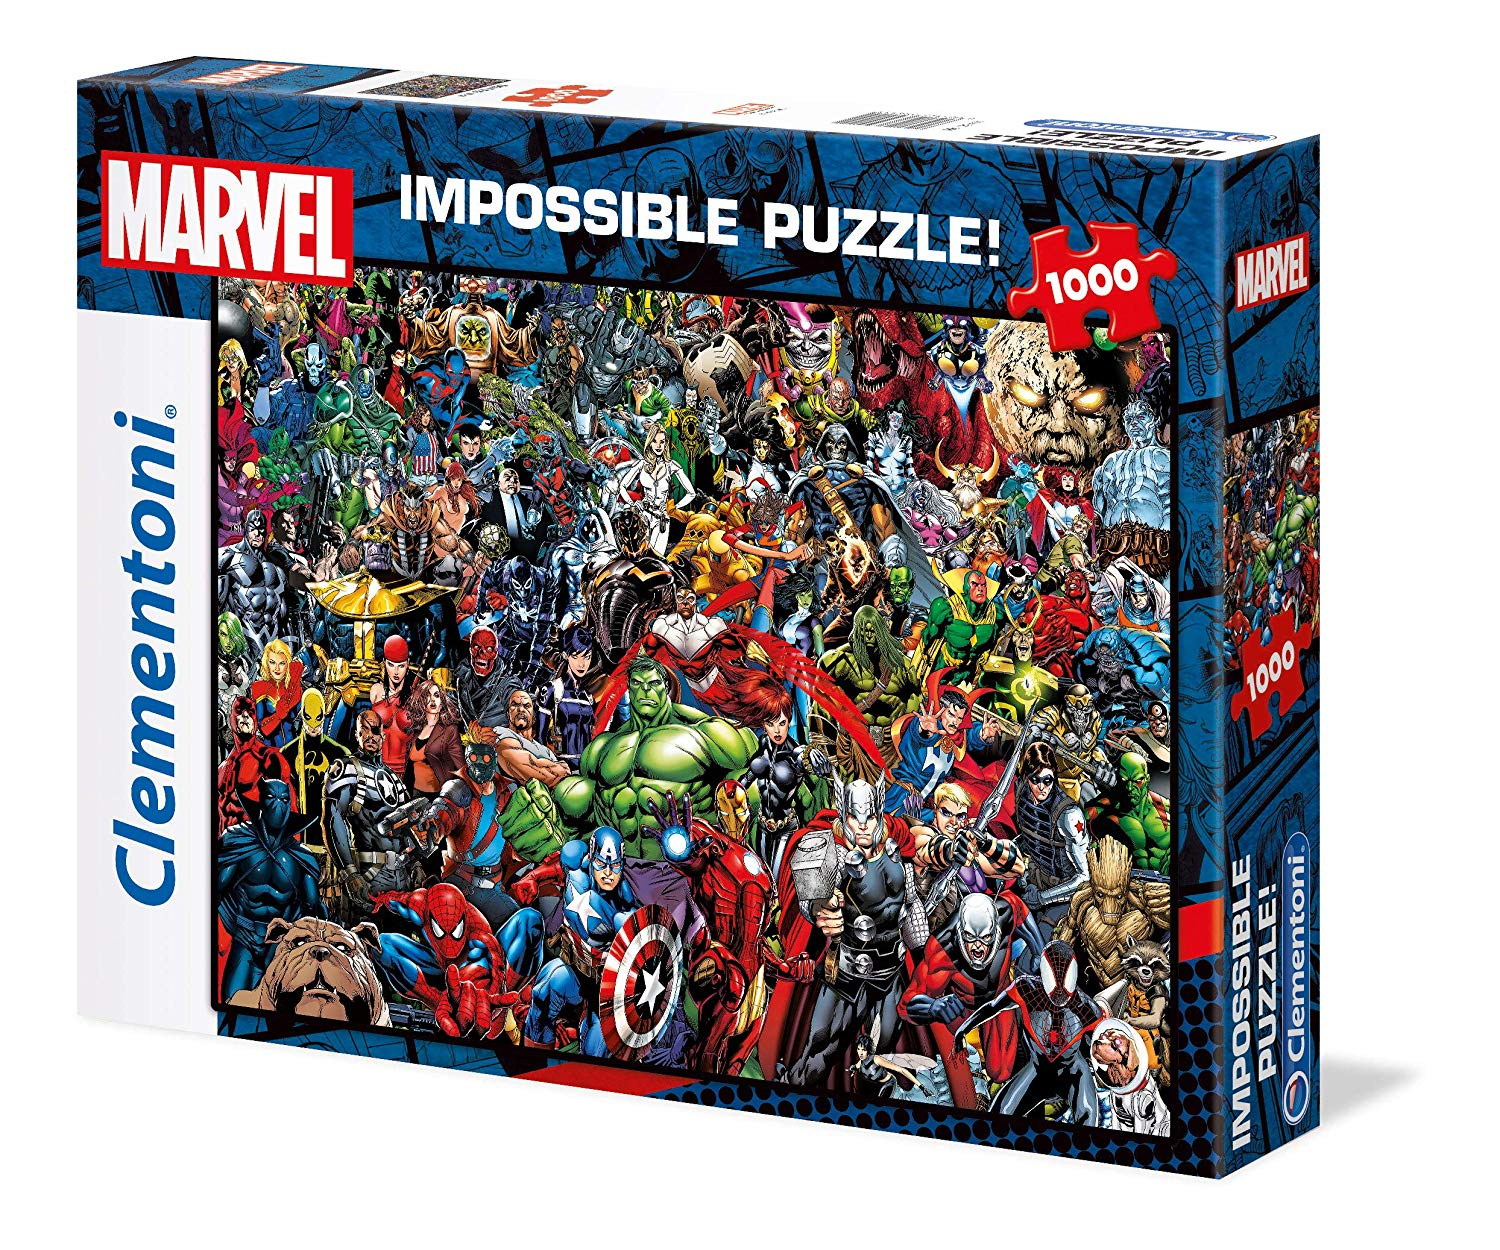
\includegraphics[width=\linewidth,height=.8\textheight]{./Figures/chapter-01/Marvel-03.jpg}
%%	\caption{}
%\end{figure}
%\end{frame}
%
%%%%%%%%%%%%%%%%%%%%%%%%%%%%%%%%%%%%%%%%%%%%%%%%%%%%%%%
%\begin{frame}
%\frametitle{DWH Use cases}
%\begin{figure}[ht]
%
%\centering
%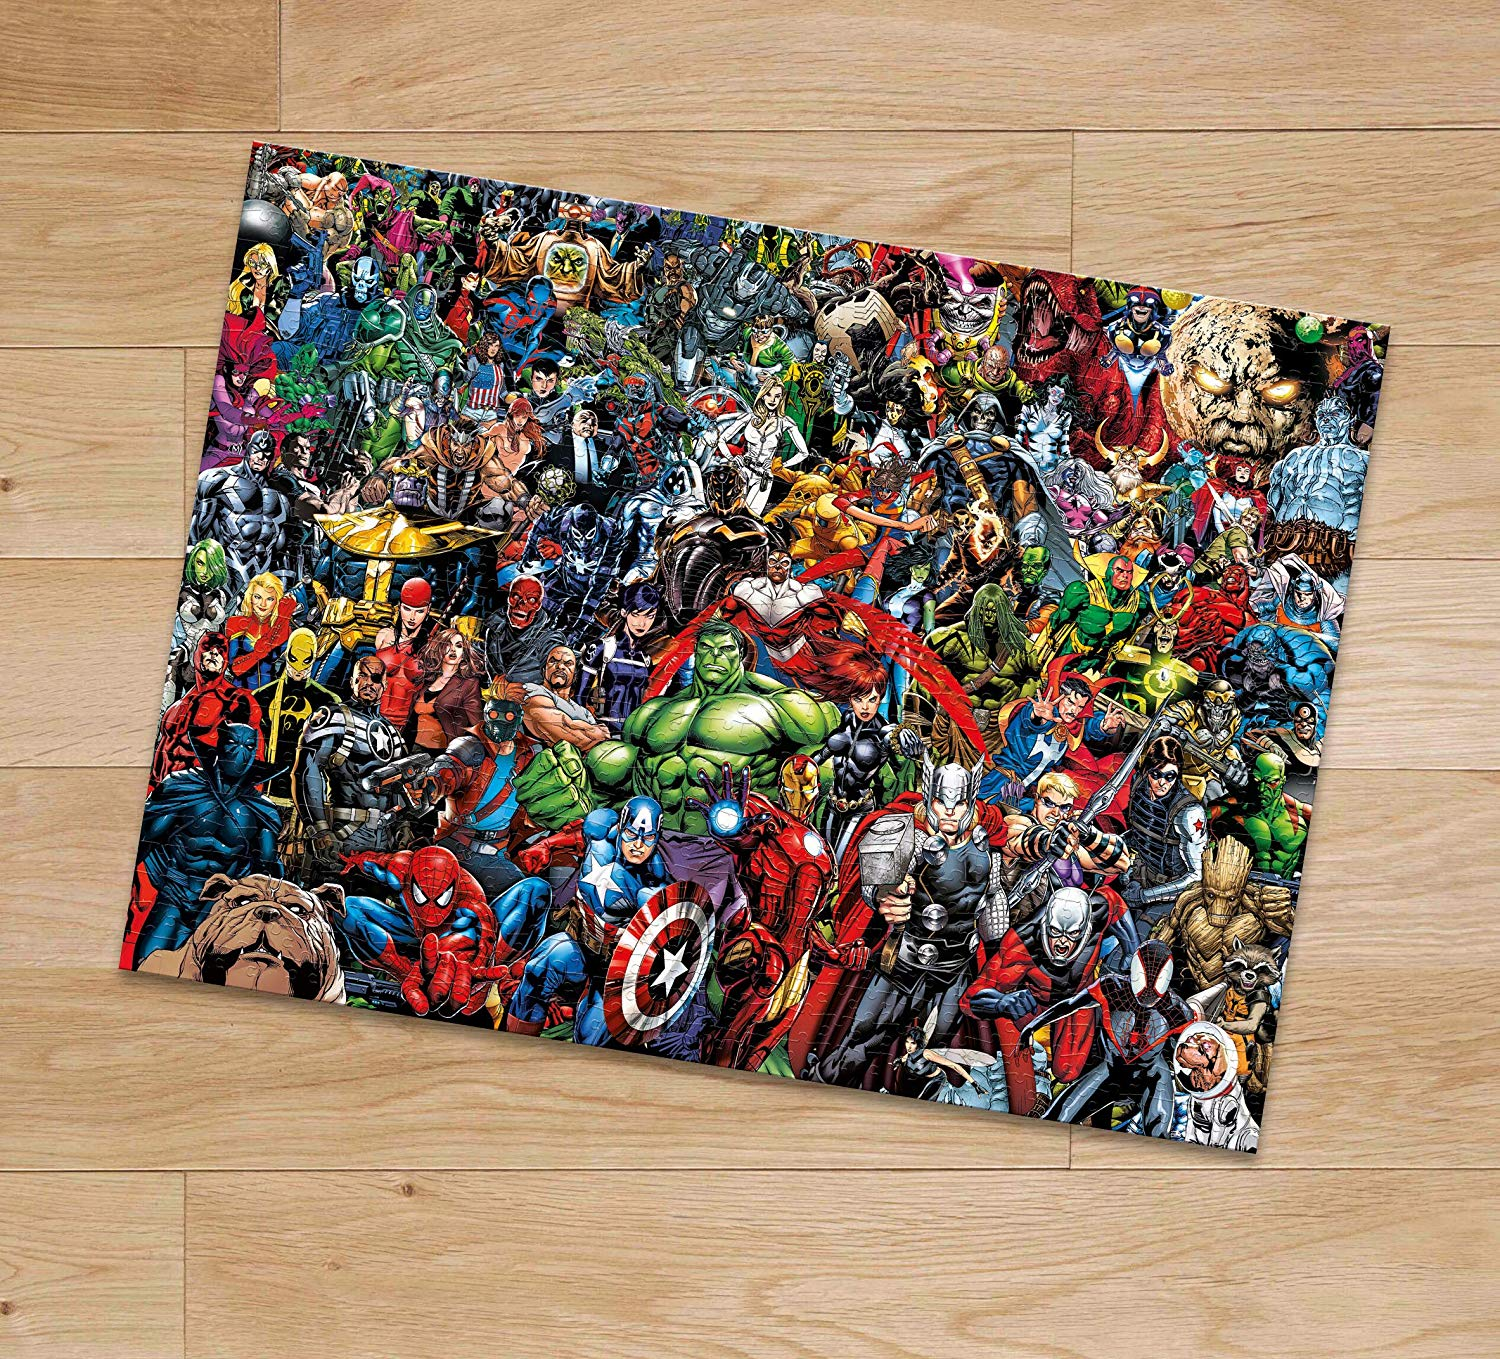
\includegraphics[width=\linewidth,height=.8\textheight]{./Figures/chapter-01/Marvel-02.jpg}
%%	\caption{}
%\end{figure}
%\end{frame}
%
%%%%%%%%%%%%%%%%%%%%%%%%%%%%%%%%%%%%%%%%%%%%%%%%%%%%%%%
%\begin{frame}
%\frametitle{DWH Use cases}
%\begin{figure}[ht]
%
%\centering
%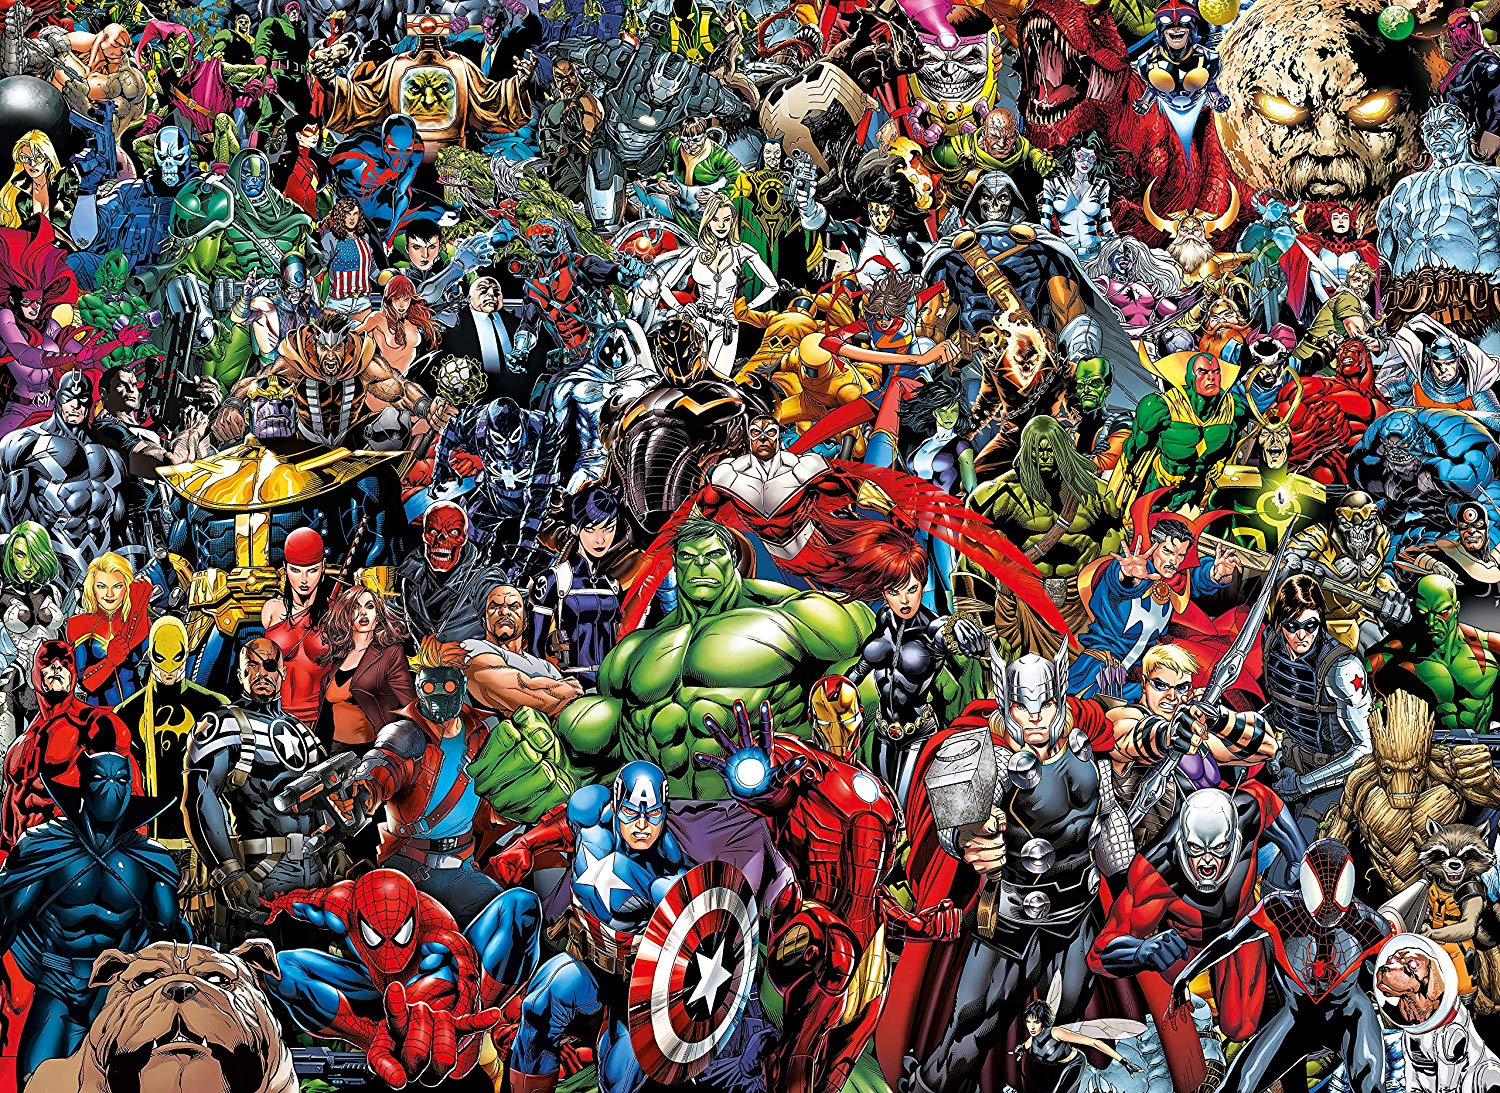
\includegraphics[width=\linewidth,height=.8\textheight]{./Figures/chapter-01/Marvel-01.jpg}
%%	\caption{}
%\end{figure}
%\end{frame}
%%%%%%%%%%%%%%%%%%%%%%%%%%%%%%%%%%%%%%%%%%%%%%%%%%%%%%%
%
%%---------------------------------------------------------
%\VideoClassification[column=2, colour=blue]
%%%%%%%%%%%%%%%%%%%%%%%%%%%%%%%%%%%%%%%%%%%%%%%%%%%%%%%
%\subsubsection{Types of DWH}
%\begin{frame}
%\frametitle{Motivation to Data Warehouse}
%Types of Data Warehouse
%\begin{description}
%\item [\textbf{Enterprise Data Warehouse (EDWH)}] It provides decision support service across the enterprise. It offers a unified approach for organizing and representing data (DWH Model). It offers data classifications according to the subject with privileges policy.
%\item [\textbf{Operational Data Store (ODS):}] is a central database that provides an up-to-date (real-time) data from multiple transnational systems for operational reporting into a single DWH.
%
%%% for real time questions and answers. call ODS using intermidiate data store. DWH is day -1 (billing & subscribtions). Oracle (Loading or headache) && CDC capture change interest column not row
%\item [\textbf{Data Mart:}] A data mart is a subset of the data warehouse. It specially designed for a particular line of business, such as sales, finance, sales or finance. In an independent data mart, data can collect directly from sources.
%\end{description}
%
%\end{frame}
%
%%%%%%%%%%%%%%%%%%%%%%%%%%%%%%%%%%%%%%%%%%%%%%%%%%%%%%%
%
%\begin{frame}
%\frametitle{DWH vs ODS vs Data Mart}
%
%
%\begin{table}[t]
%\centering	
%\resizebox{\columnwidth}{!}{%
%
%%		\centering
%\begin{tabular}{|c | c | c| c |}
%\hline
%\textbf{Metric}  & \textbf{DWH}& \textbf{ODS} & \textbf{Data Mart} \\
%\hline
%Latency & Day -1  & Real-time & Day -1 \\			
%Data level  & Transnational & Transnational & Summary \\
%Historical  & Long-term & Snapshot & Aggregated Long-Term \\
%Size & TB/PB & GB & GB/TB\\
%Orientation & Multi sources & Multi sources & Product\\
%Business Units & Multi organizational units & Product team & Business team \\
%\hline
%\end{tabular}
%%		\caption{Data Representation Combination Matrix}\label{Tab:Data_Representation_Matrix}
%}
%\end{table}
%\end{frame}
%
%
%%%%%%%%%%%%%%%%%%%%%%%%%%%%%%%%%%%%%%%%%%%%%%%%%%%%%%%%%%%%%%%%%%%%%%%%%
%\subsubsection{Use Cases of Operational DB vs DWH}
%
%\begin{frame}
%\frametitle{Use case (Operational DB)}
%
%\begin{itemize}[<+->]
%
%\item A telecommunication company named \textbf{XTec}.
%\newline
%\item They have lots of systems. One of this systems is a CRM system as example of operational DB.
%\begin{itemize}[<+->]
%
%\item The CRM system handles the customer activities with the company including (sales, change in customer plans, and other activities).
%\item This system has a backend database (MySQL).
%\item CRM team can report their sales and customer activities from their database.
%\item Product owner can take a decision based on their system backend reports.
%
%\end{itemize}
%
%\end{itemize}
%
%\end{frame}
%
%%%%%%%%%%%%%%%%%%%%%%%%%%%%%%%%%%%%%%%%%%%%%%%%%%%%%%%
%
%\begin{frame}
%\frametitle{Use case (DWH)}
%
%\begin{itemize}[<+->]
%
%\item What is the need for DWH?		
%\begin{itemize}[<+->]
%\item This company has other systems \forexample billing, charging, signaling.	
%\item They need to report information related to the CRM, billing, and signaling source systems in one report.
%\item So, they need to ingest (transfer) the data from the source systems to one single database.
%\item The decision from the DHW is a \textbf{global and strategical decision.}
%\item If the company needs to build a machine learning model which needs data from different sources. They need to load the data from a centralized database rather than read each source alone.
%\end{itemize}
%
%\end{itemize}
%
%\end{frame}
%%%%%%%%%%%%%%%%%%%%%%%%%%%%%%%%%%%%%%%%%%%%%%%%%%%%%%%
%
%
%\begin{frame}
%\frametitle{Use case (DWH)}
%\centering
%The Full picture required a DWH. However, we still need the other operational databases for product development perspective.
%
%
%\end{frame}
%%%%%%%%%%%%%%%%%%%%%%%%%%%%%%%%%%%%%%%%%%%%%%%%%%%%%%%
%
%\begin{frame}
%\frametitle{Use case (ODS)}
%\centering
%
%\begin{itemize}[<+->]
%\item Why do we need the ODS?
%\item 	How does it fit in our system?
%\end{itemize}
%
%
%\end{frame}
%%%%%%%%%%%%%%%%%%%%%%%%%%%%%%%%%%%%%%%%%%%%%%%%%%%%%%%
%
%
%%%%%%%%%%%%%%%%%%%%%%%%%%%%%%%%%%%%%%%%%%%%%%%%%%%%%%%
%
%\begin{frame}
%\frametitle{Use case (ODS)}
%\centering
%\textbf{XTec} has a call center system which handles the customer inquiries. This system requires the some data related to usage, customer information, billing details to be calculated and accumulated in \textbf{real-time} to be able to give the customer the right answer for his inquires.
%
%\end{frame}
%%%%%%%%%%%%%%%%%%%%%%%%%%%%%%%%%%%%%%%%%%%%%%%%%%%%%%%
%%%%%%%%%%%%%%%%%%%%%%%%%%%%%%%%%%%%%%%%%%%%%%%%%%%%%%%
%\begin{frame}
%\frametitle{Use case (ODS)}
%
%	\begin{itemize}[<+->]
%		\item So, What is the challenge for this system?
%			\begin{itemize}[<+->]		
%				\item It needs specific information from different source systems.
%				\item It requires to track the source system database changes or update in real-time.
%				\item It's functionality is based on the aggregate data not the transactions \forexample (It needs the total outgoing calls till time or it needs the total charging amounts from prepaid or the available limits from billing if it is postpaid).
%			\end{itemize}
%	\end{itemize}
%
%\end{frame}
%%%%%%%%%%%%%%%%%%%%%%%%%%%%%%%%%%%%%%%%%%%%%%%%%%%%%%%
%\begin{frame}
%\frametitle{Use case (ODS)}
%
%	\begin{itemize}[<+->]
%		\item ODS is based on change data capture (CDC). This approach used to determine the data change and apply action based on this change.
%		\item ODS uses the real-time aggregations to support the online systems from different source systems.
%	\end{itemize}
%\end{frame}


%---------------------------------------------------------
\VideoClassification[column=2, colour=red]
%%%%%%%%%%%%%%%%%%%%%%%%%%%%%%%%%%%%%%%%%%%%%%%%%%%%%%

\subsection{Hot vs Cold Storage}
\begin{frame}[c]
\frametitle{Hot vs Cold Storage}

%\begin{center}
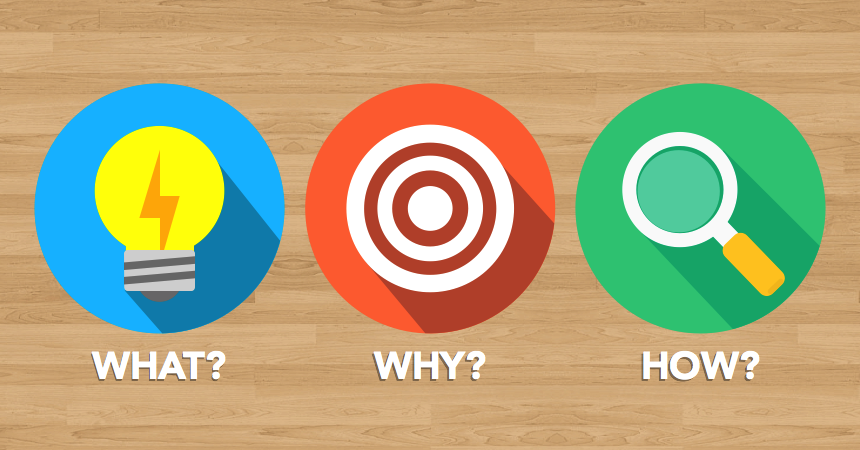
\includegraphics[width=\textheight]{./Figures/chapter-01/WWH-Thumb.png}

%\end{center}


\end{frame}
%%%%%%%%%%%%%%%%%%%%%%%%%%%%%%%%%%%%%%%%%%%%%%%%%%%%%%


\begin{frame}
\frametitle{What is multi-temperature Storage?}

\begin{wideitemize}
\item (Most of) DWH solution design has multi-temperature data management model.
\item What is the multi-temperature data management model?
\begin{itemize}[<+->]
	\item It is a data classification design which allows us to have the following characteristics
	\begin{itemize}[<+->]
		\item Fast (high performance) access on the frequent data (Hot data).
		\item Good (average performance) access to less-frequently data (warm data).
		\item Availability to access rarely accessed data (cold data).
	\end{itemize}
	\item Who is responsible for data temperature classifications?
	\begin{itemize}[<+->]
		\item Demand team, product owner, or data architect (Based on the business needs).
	\end{itemize}
\end{itemize}
\end{wideitemize}
\end{frame}

%%%%%%%%%%%%%%%%%%%%%%%%%%%%%%%%%%%%%%%%%%%%%%%%%%%%%%

\begin{frame}
\frametitle{Why do we need it?}

\begin{wideitemize}
\item Why do we need the multi-temperature data management model?
\begin{itemize}[<+->]
\item Cost reduction \blue{\faDollar \faDollar \faDollar \faDollar}
\item Performance.
\end{itemize}
\end{wideitemize}
\end{frame}
%%%%%%%%%%%%%%%%%%%%%%%%%%%%%%%%%%%%%%%%%%%%%%%%%%%%%%

\begin{frame}
\frametitle{How to implement a multi-temperature storage system? }

\begin{wideitemize}
\item How to implement the multi-temperature data management model?
\begin{itemize}[<+->]
\item Before implementation, we need to know the following:
\begin{itemize}[<+->]
\item Frequency of access
\item Data change rate.
\end{itemize}
\item Identify which storage type is suitable for the project
\begin{itemize}[<+->]
\item We store the hot data on the fast storage system.
\item Warm data (usual) stored on slightly slower storage.
\item We store the cold data on the slowest storage.
\end{itemize}
\end{itemize}
\end{wideitemize}
\end{frame}

%%%%%%%%%%%%%%%%%%%%%%%%%%%%%%%%%%%%%%%%%%%%%%%%%%%%%%

\begin{frame}
\frametitle{How to implement a multi-temperature storage system? Cont.}

\begin{wideitemize}
\item Design consideration to make the retention easily.
\begin{itemize}[<+->]
\item Table partitions need to be split based on the retention policy plan \forexample (date).
\item Summary tables (agg) need to be maintained to reduce the need for access the cold storage.
\item Backup, Recovery, and Rollback plans need to be automated and prepared/tested before moving the data.
\end{itemize}
\end{wideitemize}
\end{frame}

%%%%%%%%%%%%%%%%%%%%%%%%%%%%%%%%%%%%%%%%%%%%%%%%%%%%%%

%%%%%%%%%%%%%%%%%%%%%%%%%%%%%%%%%%%%%%%%%%%%%%%%%%%%%%

\begin{frame}
\frametitle{How to implement a multi-temperature storage system? Cont.}
\begin{wideitemize}
\item Implementation (summary):
\begin{itemize}[<+->]
\item There are lots of tools for this purpose and  categorized as follows:
\begin{itemize}
\item Enterprise.
\item Open source.
\item Cloud tools.
\end{itemize}

\end{itemize}
%Cost,Security
\end{wideitemize}
\end{frame}
%%%%%%%%%%%%%%%%%%%%%%%%%%%%%%%%%%%%%%%%%%%%%%%%%%%%%%

\begin{frame}
\frametitle{How to implement a multi-temperature storage system? Cont.}
\begin{wideitemize}
\item Enterprise \forexample:
\begin{itemize}
\item IBM InfoSphere
\item Informatica PowerCenter
\item Oracle Data Service Integrator
\item Talend Data Integration
\item Microsoft SQL
\end{itemize}
%Cost,Security
\end{wideitemize}
\end{frame}

%%%%%%%%%%%%%%%%%%%%%%%%%%%%%%%%%%%%%%%%%%%%%%%%%%%%%%

\begin{frame}
\frametitle{How to implement a multi-temperature storage system? Cont.}
\begin{wideitemize}
\item Open source \forexample:
\begin{itemize}
\item Apache NiFi*
\item CloverETL
\item Pentaho
\item Talend Open Studio*
\end{itemize}
\end{wideitemize}
\end{frame}

%%%%%%%%%%%%%%%%%%%%%%%%%%%%%%%%%%%%%%%%%%%%%%%%%%%%%%

\begin{frame}
\frametitle{How to implement a multi-temperature storage system? Cont.}
\begin{wideitemize}
\item Cloud tools \forexample:
\begin{itemize}
\item AWS Migration Services.
\item Azure Migration Tools.
\item Google Migration Services/Velostrata.
\end{itemize}
\item Some cloud providers offer physical data movement services.
\item How to choose the most suitable storage type for your project/organization?
%Cost,Security
\end{wideitemize}
\end{frame}
%---------------------------------------------------------
\VideoClassification[column=2, colour=red]
%%%%%%%%%%%%%%%%%%%%%%%%%%%%%%%%%%%%%%%%%%%%%%%%%%%%%%
\subsection{DWH Characteristics}
\begin{frame}
    \frametitle{DWH Characteristics}
    %these is not a definitions, we just show the meaning and the understanding.
    \begin{wideitemize}
        \item The characteristics of DWH:
        \begin{wideitemize}
        	\item Integrated: \textit{DWH is an integrated environment which allows us to
        	integrate different source systems. Data are modeled (organized) in a unified manner}.%regardless of the original source
        	
        	\item Time-Variant: \textit{Data modeled (organized) based on periods
        	(hourly, daily, weekly, monthly, quarterly, yearly)}.
        	
        	\item Subject-oriented: \textit{DWH main target is to support business needs for
        	the whole organization including (decision-makers, departments, and
        	specific user requirements)}.
        	
        	\item Non-Volatile: \textit{It refers to the data that erased or deleted (It could be archived and retrieved when needed). Data can be accumulated daily the new snapshots (refreshed at based on the source system interval.  \faArrowCircleORight \space It could be updated daily, weekly, and monthly)}.
        \end{wideitemize}
    \end{wideitemize}
\end{frame}
%%%%%%%%%%%%%%%%%%%%%%%%%%%%%%%%%%%%%%%%%%%%%%%%%%%%%%
\subsection{DWH Architecture}
\begin{frame}
\frametitle{DWH Architecture Overview}
	\begin{tikzpicture}[every label/.append style={font=\tiny},regentonne/.style={cylinder,aspect=.7,draw,shape border rotate=90}]
		%\draw[step=.5cm,gray,very thin] (-2,-1) grid (9.5,6);
		%SS recatangle
		\filldraw[draw=blue,thick,rounded corners,fill=white] (-2,-1) rectangle (0.2,6);

		%ETL recatangle		
		\filldraw[draw=Maroon,thick,rounded corners,fill=white] (.4,0) rectangle (2.5,6);
		
		%EDW
		\filldraw[draw=OliveGreen,thick,rounded corners,fill=white] (2.7,0) rectangle (7.7,6);
		
		%BI LAYER
		\filldraw[draw=mauve,thick,rounded corners,fill=white] (7.9,0) rectangle (9.5,6);

		%Metadata LAYER
		\filldraw[draw=ballblue,thick,rounded corners,fill=white] (.4,-1.2) rectangle (9.5,-.7);

		%User Access LAYER
		\filldraw[draw=black,thick,rounded corners,fill=white] (.4,-.6) rectangle (9.5,-.1);

		
   	    \node[text width=2cm,font=\scriptsize] at (-.9,5.6) {Source Systems};
		\node[database,label=below:CRM] (s1) at (-1,5) {};
		\node[database,label=below:ERP] (s2) at (-1,4) {};
		\node[database,label=below:MobileApp] (s3) at (-1,3) {};		
		\node[database,label=below:Billing] (s4) at (-1,2) {};		
		\node[database,label=below:WebApp] (s5) at (-1,1) {};						
		\node[database,label=below:Other] (s6) at (-1,0) {};				
		
		\draw[line width=0.25mm, blue] (s1) -- ([xshift=.5cm]s1.east) -- ([xshift=.5cm]s2.east) -- (s2)  -- ([xshift=.5cm]s2.east) -- ([xshift=.5cm]s3.east) -- (s3)-- ([xshift=.5cm]s3.east) -- ([xshift=.5cm]s4.east) -- (s4) -- ([xshift=.5cm]s4.east) --  ([xshift=.5cm]s5.east) -- (s5) --  ([xshift=.5cm]s5.east) -- ([xshift=.5cm]s6.east) -- (s6);
	
		%connection arrow
		\draw[->,line width=0.5mm, black] ([xshift=.5cm,yshift=-.5cm]s3.east) -- ([xshift=1.45cm,yshift=-.5cm]s3.east) ;		

		
		%ETL
   	    \node[text width=2cm,font=\scriptsize] at (2.2,5.6) {ETL};
        \pic[draw,fill=Maroon]          (etlS) at (1.45,4.3)   {gear={0.08}{17}{15}};
        \pic[draw,fill=uiborange]       (etlM) at (1.45,2.5)   {gear={0.08}{17}{15}};
        \pic[draw,fill=mygreen]         (etlB) at (1.45,.8)   {gear={0.08}{17}{15}};
   		\draw[line width=0.25mm, gray] (2.03,4.3) -- (2.4,4.3);
  		\draw[line width=0.25mm, gray] (2.03,2.5) -- (2.4,2.5);
  		\draw[line width=0.25mm, gray] (2.03,.8) -- (2.4,0.8);
  		\draw[line width=0.25mm, gray] (2.4,4.3) -- (2.4,0.8);  		
		%connection arrow	
  		\draw[->,line width=0.5mm, black] (2.4,2.5) -- (3.3,2.5);
   		
		%EDW
   	    \node[text width=4.5cm,font=\scriptsize] at (5.3,5.6) {Enterprise Data Warehouse (EDW)};
     	\node[database,label=below:DWH,database radius=.7cm,database segment height=.4cm] (A)  at (4,2.6) {};
     	\node[database,label=below:Data Mart,database radius=.4cm,database segment height=.2cm]  (B)  at (6.5,4) {};     	
     	\node[database,label=below:Data Mart,database radius=.4cm,database segment height=.2cm]  (C)  at (6.5,2.5) {};
     	\node[database,label=below:Data Mart,database radius=.4cm,database segment height=.2cm]  (D)  at (6.5,1) {};     	
     	\node[database,label=below:Operational Data Store,database radius=.6cm,database segment height=.3cm] (E) at (4,4.6) {};
    
       \draw[line width=0.25mm,alizarin,->] (A) -- (B);
       \draw[line width=0.25mm,alizarin,->] (A) -- (C);
       \draw[line width=0.25mm,alizarin,->] (A) -- (D);
       \draw[line width=0.25mm,alizarin,->] (E) -- (A);

       \draw[line width=0.25mm,alizarin] (7.3,.9) -- (7.3,4);
       
       \draw[line width=0.25mm,alizarin] (6.9,4) -- (7.3,4);
       \draw[line width=0.25mm,alizarin] (6.9,2.5) -- (7.3,2.5);
       \draw[line width=0.25mm,alizarin] (6.9,.9) -- (7.3,.9);
       
       \draw[line width=0.5mm,black,->] (7.3,2.5) -- (8,2.5);
       
		%BI LAYER
		\node[text width=1.3cm,font=\scriptsize] at (8.8,5.6) {BI Layer};
		\node[inner sep=0pt] (rep) at (8.7,4.6) {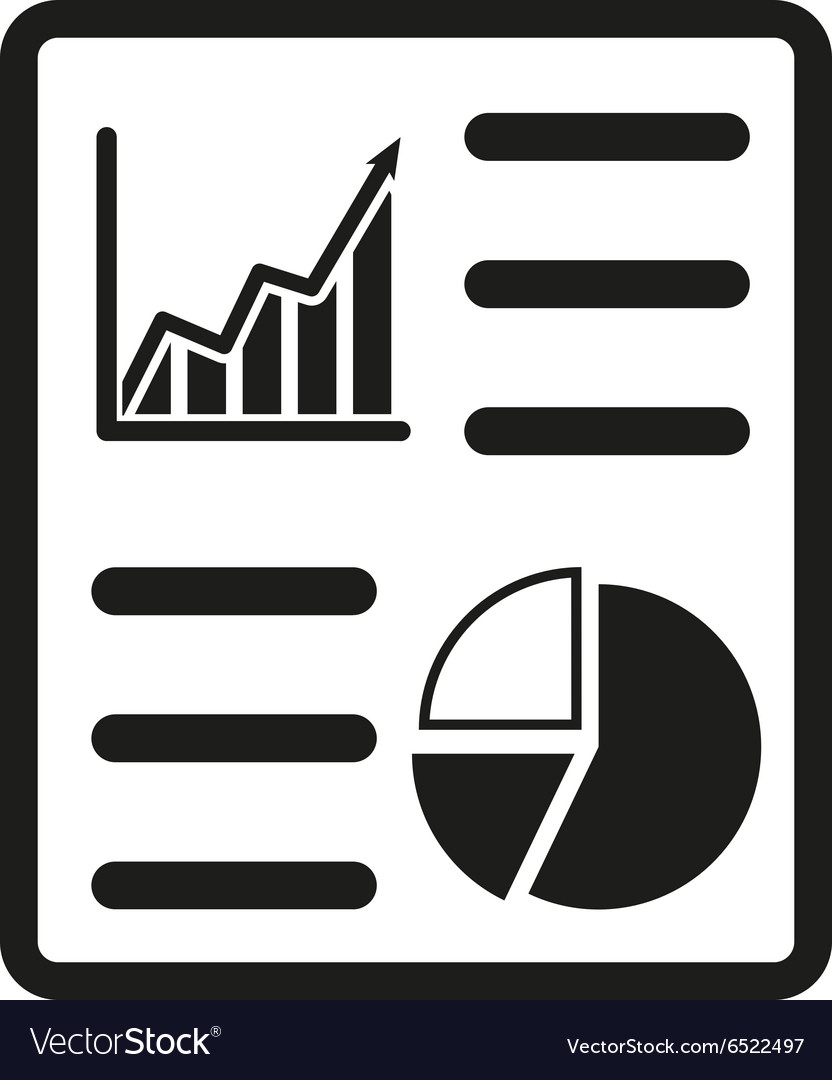
\includegraphics[width=.1\textwidth,height=.1\textheight]{./Figures/chapter-01/report.png}};
		\node[yshift=.4cm,below of=rep] {{\tiny Reporting}};
		\node (io) at (8.7,2.5) [io] {{\tiny Analytics}}; 		
		\node (start) at (8.7,0.5) [startstop] {{\tiny Integrations}}; 

		%MDM
		\node at (4.5,-.4) {Metadata Repository Management (MDM)};
		
		%Access Layer
		\node at (4.5,-1) {User Access Management \faExpeditedssl};
		
	\end{tikzpicture}

\end{frame}
%%%%%%%%%%%%%%%%%%%%%%%%%%%%%%%%%%%%%%%%%%%%%%%%%%%%%%
\begin{frame}
\frametitle{DWH Architecture Layers}

\begin{wideitemize}
	\item DWH architecture contains the following layers:
	\begin{itemize}[<+->]
		\item Source system layer.
		\item Extraction layer.
		\item Staging Area.
		\item Data Modeling.
		\item ETL layer.
		\item Storage layer.
		\item Reporting (UI) layer.
		\item Metadata layer.
		\item System operations layer.
	\end{itemize}
\end{wideitemize}

\end{frame}
\VideoClassification[column=2, colour=blue]
%%%%%%%%%%%%%%%%%%%%%%%%%%%%%%%%%%%%%%%%%%%%%%%%%%%%%%
\subsubsection{Source System Integration Process}
\begin{frame}
    \frametitle{Source System Integration Process}
    \begin{itemize}[<+->]
        \item In some companies, they hire or dedicate a team for this part (business analyst, system analyst, data analyst, or demand team).
        \item Before we start, we need to document all the communications into any format.
		\begin{itemize}
            \item Confluence pages, Word, or Excel sheet.
            \item Make the discussion online and put comments to make the history available always.
			\item We need to clarify all the tasks and what is the expected output, \forexample (analysis means to document data structure, format, column names, etc.).
        \end{itemize}
    \end{itemize}

\end{frame}

%%%%%%%%%%%%%%%%%%%%%%%%%%%%%%%%%%%%%%%%%%%%%%%%%%%%%%
\begin{frame}
    \frametitle{Source System Integration Process}
    \begin{itemize}[<+->]
        \item  Requirements gathering. % or business need (It could be DWH unification).
        \item  Identify the stakeholders (Data owner(s)).
        \item  Data Analysis includes but not only (format, latency, and column definitions).
        \item  Check the source system access and perform connectivity assessment.
        \item  Initiate the technical discussion about the best way to ingest the data.
        \item  Data Ingestion method and format.
        \item  Sign or confirmation for every point between the stakeholders.
        \item  \blue{This layer deliver a data analysis (Source system interface ) document}.
    \end{itemize}

\end{frame}


%%%%%%%%%%%%%%%%%%%%%%%%%%%%%%%%%%%%%%%%%%%%%%%%%%%%%%
\VideoClassification[column=2, colour=blue]
\subsubsection{Extraction Layer}

\begin{frame}
    \frametitle{Extraction Layer}
    \begin{itemize}[<+->]
		\item In some companies, they hire or dedicate a team for this part (extraction or ingestion team), but in other companies, it is part of the data engineering team.
		\item This layer takes the output analysis and decisions from the previous layer (source system analysis) and implement the extraction (quality from the previous team output highly affect this team).
		\item There is a lot of consideration this team needs to take care of or deal with, but we can summarize it in the following:
		\begin{itemize}[<+->]
			\item Data latency analysis as it affects the tool and the methodology (stream or batch).
			\item Data extraction method (push or pull).
			\item Data size and format compared with the available resources for this project.
	    \end{itemize}
        \item \blue{This layer output is a minimal data cleansing (no transformation) into the staging/landing layer}.
    \end{itemize}
\end{frame}

%%%%%%%%%%%%%%%%%%%%%%%%%%%%%%%%%%%%%%%%%%%%%%%%%%%%%%

\subsubsection{Staging Layer}
\begin{frame}
    \frametitle{Staging Layer}
    \begin{itemize}[<+->]
        \item This layer handled by the same team who own the \blue{storage part} in most of the organizations.
        \item Segregation of this layer if it uses different storage type or multi-teams access this layer for a different purpose \forexample (Kafka)\\ \red{\textit{\faBullhorn Kafka is not a storage layer, but it could be used as a landing layer or data persistence layer}}.
        \item All the ETL layers are working on top of this layer.
        \item The decision of the storage type is based on the use case and the data.

    \end{itemize}

\end{frame}
\VideoClassification[column=2, colour=red]
%%%%%%%%%%%%%%%%%%%%%%%%%%%%%%%%%%%%%%%%%%%%%%%%%%%%%%
%%%%%%%%%%%%%%%%%%%%%%%%%%%%%%%%%%%%%%%%%%%%%%%%%%%%%%
%%%%%%%%%%%%%%%%%%%%%%%%%%%%%%%%%%%%%%%%%%%%%%%%%%%%%%
\VideoClassification[column=1, colour=red]
\subsubsection{Data Modeling}


\begin{frame}
    \frametitle{Data Modeling Objective}
    \begin{itemize}[<+->]
        \item Explain what data modeling is and its roles?
        \item Be aware of its importance.
        \item Explore different types of data modeling.
        \item \blue{We target to explain the main components and types, and for more details, it could be found in the appendix videos.}.
    \end{itemize}

\end{frame}

%%%%%%%%%%%%%%%%%%%%%%%%%%%%%%%%%%%%%%%%%%%%%%%%%%%%%%

\begin{frame}
    \frametitle{What is data model?}
	The data model
    \begin{itemize}[<+->]
        \item is An abstract model that organizes elements of data.
        \item It describes the objects, entities, and data structure properties, semantic, and constraint.
        \item It formalizes the relationship between entities.
        \item It describes how the application (report) API data manipulation.
        \item It describes the conceptual design of a business or an application with its flow, logic, semantic information (rules), and how things are done.
        \item It refers to a set of concepts used in defining such as entities, attributes, relations, or tables.
    \end{itemize}
\end{frame}

%%%%%%%%%%%%%%%%%%%%%%%%%%%%%%%%%%%%%%%%%%%%%%%%%%%%%%
\begin{frame}
    \frametitle{What is data model?}

    \begin{columns}

        \column{0.4\textwidth}
        Data model is not
        \begin{itemize}[<+->]
            \item a science.
            \item a static design for each organization.
            \item a type of database.
            \item a new invention which needs to be done for each project.
            %ex: sldm teradata model
        \end{itemize}


        \column{0.45\textwidth}
        Data model is
        \begin{itemize}[<+->]
            \item a general concept that leads to build full architecture.
            \item an engineering design practices.
            \item different based on the use case and the database type.
            \item customizable, and we can utilize some of the ready built architecture.
            \item affecting information reporting performance.
        \end{itemize}

        \column{0.2\textwidth}
    \end{columns}

\end{frame}

%%%%%%%%%%%%%%%%%%%%%%%%%%%%%%%%%%%%%%%%%%%%%%%%%%%%%%

\begin{frame}
    \frametitle{What is data model?}
    The data model is
    \begin{itemize}[<+->]
        \item The fist part before starting integration with any new source system.
        \item The connection layer between business requirements and technical design.
        \item It is also the translation between logical and physical layer.
        \item It is unified across all systems and has the same patterns and practices.
        \item It engaged with any source systems integration from the early stages.
        \item \blue{This stage output is a data model design document or mapping sheet}.
    \end{itemize}
\end{frame}

%%%%%%%%%%%%%%%%%%%%%%%%%%%%%%%%%%%%%%%%%%%%%%%%%%%%%%

\begin{frame}
    \frametitle{Why does the data model are important?}
    \begin{wideitemize}
        \item Data models are currently affecting software design.
        \item It decides how engineers think about the problem they are solving.
    \end{wideitemize}
\end{frame}

%%%%%%%%%%%%%%%%%%%%%%%%%%%%%%%%%%%%%%%%%%%%%%%%%%%%%%
\begin{frame}
    \frametitle{Data Model Design vs Implementation}
    %Replace it by photo
    \begin{itemize}[<+->]
        \item If you need to build a home, so, how do we design this home?
        \begin{itemize}[<+->]
            \item Determine if the home is one level or multi-level and decide man bedrooms and bathrooms for each floor. (User needs)
            \item Hire an architect to put the architecture in more detailed way \forexample the size for each room, the distribution of the wires, where the plumbing fixtures will be placed, etc. (Architecture phase)
            \item Decide the decorations, colors for each room, carpets, etc.
        \end{itemize}
        \item What do we do for the implementation?
        \begin{itemize}[<+->]
            \item Hire a contractor to build (implement the design) the home.
            \item This phase implement the design, but it also includes some detail related to the real way to build the tools and the material (Physical Design).
        \end{itemize}
    \end{itemize}
\end{frame}

%%%%%%%%%%%%%%%%%%%%%%%%%%%%%%%%%%%%%%%%%%%%%%%%%%%%%%
\midTitle{Data Model: Elements of Data Model}
\begin{frame}
    \frametitle{Elements of Data Model}
    \begin{description}[<+->]
        \item[Facts] are the measurements/metrics or facts from the business process \forexample (Telecom industry, measurement would be the count of daily/hourly usage per customer). We could consider facts as the source of reporting for the business.
        %measure and ids when,where
        \item[Dimensions] provide the context surrounding a business process event. In simple terms, they give who, what, where the fact, \forexample (Telecom industry, for the fact daily usage, dimensions would be customer\_id, location\_id).
        
        \item[Attributes] are the various characteristics of the dimension. In the previous examples, the attributes can be customer details (from customer\_id get the gender, age, nationality, etc.).
        %Attributes are used to search, filter, or classify facts. Dimension Tables contain Attributes
        %	Facts include dimensions, dimensions include attributes
    \end{description}
\end{frame}

%%%%%%%%%%%%%%%%%%%%%%%%%%%%%%%%%%%%%%%%%%%%%%%%%%%%%%
\begin{frame}
    \frametitle{Elements of Dimensional Data Model}
    \begin{description}[<+->]
        \item[Fact Table] is a primary table in a dimensional model. A Fact Table contains (Measurements/facts and Foreign key to \textit{dimension table}). It located at the center of a star or snowflake schema and surrounded by dimensions.
        %	contains only ids customer, date, location ids  to get this ids go to the diem
        %granuality for levels / agg up down
        \item[Dimension table] contains dimensions of a fact and business reference data. They are joined to fact table via a foreign key. Dimension tables are de-normalized tables. It connected to the fact table and located at the edges of the star or snowflake schema.

    \end{description}
\end{frame}

%%%%%%%%%%%%%%%%%%%%%%%%%%%%%%%%%%%%%%%%%%%%%%%%%%%%%%
\begin{frame}
    \frametitle{Example of Data Model}

    
\resizebox{\columnwidth}{!}{%
\begin{tikzpicture}[every node/.style={font=\ttfamily}, node distance=1.4in,scale=.75, every node/.style={scale=0.75}]
%https://tex.stackexchange.com/questions/133754/creating-crows-foot-style-e-r-diagrams-rather-than-chen-style-ones
\matrix  [entity=Usage, entity anchor=Usage-id]  {
	\properties{
		id,
		cust-id (FK),
		cal-id (FK), 
		loc-id (FK),
		promo-id (FK),
		date-id (FK),
		TotalInCalls (agg),
		TotalOutCalls (agg),
		TotalAmount (agg)
	}
};


\matrix  [entity=CellLookup, above left=of Usage-id, entity anchor=CellLookup-id]  {
	\properties{
		id,
		celltype,
		vendorname,
		street,
		city,
		state,
		zip
	}
};
\matrix  [entity=Promotion, below left=of Usage-id,yshift=10ex, entity anchor=Promotion-id]  {
	\properties{
		id,
		promotype,
		promodesc,
		value,
		startdate,
		enddate
	}
};

\matrix [entity=CustomerProfile, below right=of Usage-id,yshift=10ex, entity anchor=CustomerProfile-id]  {
	\properties{
		id, 
		gender, 
		age, 
		nationality,
		firstname,
		lastname
	}
};


\matrix  [entity=Calendar, above right=of Usage-id, entity anchor=Calendar-id]  {
	\properties{
		id,
		date,
		day,
		week,
		month,
		qtr,
		year
	}
};

\draw [one to one] (Usage-id)  to (CustomerProfile-id);
\draw [one to one] (Usage-id)  to (Calendar-id);
\draw [one to one] (Usage-id)  to (CellLookup-id);
\draw [one to one] (Usage-id)  to (Promotion-id);

\end{tikzpicture}
}
\end{frame}

%%%%%%%%%%%%%%%%%%%%%%%%%%%%%%%%%%%%%%%%%%%%%%%%%%%%%%
\midTitle{Data Model: Elements of Data Model}
\begin{frame}
	\frametitle{Elements of Data Model}
		Dimensional model life cycle:
	    \begin{itemize}[<+->]
			\item Gathering Requirements (Source Driven, Business/User Driven).
			\item Identify granularity of the facts
			\item Identify the dimensions
			\item Identify the facts
	    \end{itemize}	
\end{frame}
%%%%%%%%%%%%%%%%%%%%%%%%%%%%%%%%%%%%%%%%%%%%%%%%%%%%%%

\begin{frame}
\frametitle{Dimensions Types}
	\begin{enumerate}[<+->]
		\item Conformed Dimension.
		\item Degenerate Dimension.
		\item Junk Dimension (Garbage Dimension).
		\item Role-Playing Dimension.
		\item Outrigger Dimension.
		\item Snowflake Dimension.
		\item Shrunken Rollup Dimension.
		\item Swappable Dimension.
		\item Slowly changing Dimension.
		\item Fast Changing Dimension (Mini Dimension).
		\item Heterogenous Dimensions
		\item Multi-valued dimensions
	\end{enumerate}
\end{frame}
%%%%%%%%%%%%%%%%%%%%%%%%%%%%%%%%%%%%%%%%%%%%%%%%%%%%%%
\VideoClassification[column=1, colour=blue]
%%%%%%%%%%%%%%%%%%%%%%%%%%%%%%%%%%%%%%%%%%%%%%%%%%%%%%
\midTitle{Dimensions Types: Conformed Dimension}
\begin{frame}
    \frametitle{Conformed Dimensions}
    %https://www.guru99.com/dimensional-model-data-warehouse.html
    %The dimension can also contain one or more hierarchical relationships
    \begin{description}[<+->]
        \item[Conformed Dimensions]    the dimension which is \underline{\textit{identical}} and has the \underline{\textit{same meaning}} across many fact tables which it relates and used in different areas of the warehouse.
        \begin{example}
            \begin{itemize}[<+->]
                \item \underline{\textbf{(Date as a Key)}}: if we have a date column across many facts, we could use the date as key in all tables. So, it should be a unified format.
                \item \underline{\textbf{(Product-Id as a Key)}}: if we have a product name which could vary between systems
                \forexample (upper/lower) We can create a dimension table for the product details and use product id unified across fact tables.
            \end{itemize}
        \end{example}
    \end{description}
\end{frame}
%%%%%%%%%%%%%%%%%%%%%%%%%%%%%%%%%%%%%%%%%%%%%%%%%%%%%%
\VideoClassification[column=1, colour=blue]
%%%%%%%%%%%%%%%%%%%%%%%%%%%%%%%%%%%%%%%%%%%%%%%%%%%%%%
\midTitle{Dimensions Types: Degenerate Dimension}
\begin{frame}
	\frametitle{Degenerate Dimensions}
	%https://www.guru99.com/dimensional-model-data-warehouse.html
	\begin{itemize}[<+->]
		\item Degenerate Dimensions
		\begin{itemize}[<+->]
			\item Dimension Key without corresponding dimension table.% (Not a fact and not an attribute)
			\item Stored in fact table.
			%This kind of dimension does not have its dimension as it is derived from the fact table.
			\item It used to provide a grouping for business cases.
		\end{itemize}
	\end{itemize}
\end{frame}
%%%%%%%%%%%%%%%%%%%%%%%%%%%%%%%%%%%%%%%%%%%%%%%%%%%%%%
\VideoClassification[column=1, colour=blue]
%%%%%%%%%%%%%%%%%%%%%%%%%%%%%%%%%%%%%%%%%%%%%%%%%%%%%%
\begin{frame}
	\frametitle{Degenerate Dimension}
	%https://www.guru99.com/dimensional-model-data-warehouse.html
	\begin{itemize}
		\item Degenerate Dimensions
		\begin{itemize}
			\item Dimension Key without corresponding dimension table.% (Not a fact and not an attribute)
			\item Stored in fact table.
			\item It used to provide a grouping for business cases.
			%This kind of dimension does not have its dimension as it is derived from the fact table.
		\end{itemize}
	\end{itemize}
	\centering
	\begin{tikzpicture}[every node/.style={font=\ttfamily}, node distance=1.4in,scale=.6, every node/.style={scale=0.6}]
    \matrix  [entity=OrderDetail, entity anchor=OrderDetail-OrderID]  {
    \properties{
    OrderID,
    OrderDate (FK),
    ProductID (FK),
    Quantity,
    Amount
    }
    };
\end{tikzpicture}

	
	\begin{table}[t]
		\centering
		\sffamily
		\begin{tabular}{|a | l | l | l | l|}
			\hline
			OrderID  & OrderDate & ProductID & Quantity & Amount\\
			\hline
			\hline
			%\rowcolor{LightCyan}
			123 & 123456789 & 111 & 2 & 120.45\\
			123 & 123456789 & 222 & 5 & 10.45\\
			%\rowcolor{myorange}
			\hline
			\hline
			431 & 98765122 & 333 & 1 & 15.45\\
			431 & 98765122 & 555 & 6 & 4.45\\
			\hline
		\end{tabular}
	\end{table}
\end{frame}

%%%%%%%%%%%%%%%%%%%%%%%%%%%%%%%%%%%%%%%%%%%%%%%%%%%%%%
\VideoClassification[column=1, colour=blue]
%%%%%%%%%%%%%%%%%%%%%%%%%%%%%%%%%%%%%%%%%%%%%%%%%%%%%%
\midTitle{Dimensions Types: Junk Dimension (Garbage Dimension)}
\begin{frame}
    \frametitle{Junk Dimension}
    \begin{itemize}[<+->]
        %junk assume we have multi flags we will collect them as one id
        \item It used to reduce the number of dimensions (low-cardinality columns) in the dimensional model and reduce the number of columns in the fact table. It is a collection of random transnational codes, flags, or text attributes.
        \item It optimizes space as fact tables should not include low-cardinality or text fields. It mainly includes measures, foreign keys, and degenerate dimension keys.
    \end{itemize}
\end{frame}
%%%%%%%%%%%%%%%%%%%%%%%%%%%%%%%%%%%%%%%%%%%%%%%%%%%%%%
\begin{frame}
    \frametitle{Junk Dimension}
    %\resizebox{\columnwidth}{!}{%
\begin{tikzpicture}[every node/.style={font=\ttfamily}, node distance=1.4in,scale=.6, every node/.style={scale=0.6}]
\matrix  [entity=Car, entity anchor=Car-id]  {
	\properties{
		id,
		colour-id (FK),
		body-id (FK)
	}
};


\matrix  [entity=Colour, left=of Car-id, entity anchor=Colour-id]  {
	\properties{
		id,
		colourname
	}
};
\matrix  [entity=Body, right=of Car-id,xshift=-15ex,entity anchor=Body-id]  {
	\properties{
		id,
		bodyname
	}
};
\draw (-10,1) -- (8,1) node[blue,draw=red, ultra thin, minimum size=1cm] [above,pos=0.5] {Design without junk DIM};
\draw [one to one] (Car-id)  to (Colour-id);
\draw [one to one] (Car-id)  to (Body-id);
\end{tikzpicture}
%}

%\resizebox{\columnwidth}{!}{%
	\begin{tikzpicture}[every node/.style={font=\ttfamily}, node distance=1.4in,scale=.6, every node/.style={scale=0.6}]
	
	\matrix  [entity=Car, entity anchor=Car-id]  {
		\properties{
			id,
			car-attirbute-id (FK),
		}
	};	

	\matrix  [entity=Car-Attributes, left=of Car-id, entity anchor=Car-Attributes-id]  {
		\properties{
			id,
			colourname,
			bodyname
		}
	};
	\draw (-10,1) -- (8,1) node[blue,draw=red, ultra thin, minimum size=1cm] [above,pos=0.49] {Design with junk DIM};
	\draw [one to one] (Car-id)  to (Car-Attributes-id);
	\end{tikzpicture}
%}

\end{frame}
%%%%%%%%%%%%%%%%%%%%%%%%%%%%%%%%%%%%%%%%%%%%%%%%%%%%%%
\begin{frame}
	\frametitle{Junk Dimension}

	\begin{block}{Junk Dimension Table Size}
		\begin{itemize}
			\item We must split the Junk dimension into more dimensions in case the size grows by the time.
			\item It is easy to calculate the expected number of rows as it is the total number of combinations between the low-cardinality attributes; \forexample 3 columns each have 3 values total = 3 * 3 = 9.
		\end{itemize}
	\end{block}
	
\end{frame}
%%%%%%%%%%%%%%%%%%%%%%%%%%%%%%%%%%%%%%%%%%%%%%%%%%%%%%
\VideoClassification[column=1, colour=blue]
%%%%%%%%%%%%%%%%%%%%%%%%%%%%%%%%%%%%%%%%%%%%%%%%%%%%%%
\midTitle{Dimensions Types: Role-Playing Dimension}
\begin{frame}
    \frametitle{Role-Playing Dimension}
    \begin{description}
        \item [Role-Playing Dimensions (Re-usable Dimension)] A single physical dimension helps to reference multiple times in a fact table as each reference linking to a logically distinct role for the dimension.
    \end{description}
    \centering
    \begin{tikzpicture}[every node/.style={font=\ttfamily}, node distance=1.4in,scale=.6, every node/.style={scale=0.6}]

    \matrix  [entity=OrderDetail, entity anchor=OrderDetail-OrderID]  {
        \properties{
        OrderID,
        OrderDate (FK),
        ShippedDate (FK),
        DeliveryDate (FK),
        ExpiryDate (FK)
        }
    };
    \matrix  [entity=Calendar, right=of OrderDetail-OrderID, entity anchor=Calendar-id] {
        \properties{
        id,
        date,
        day,
        week,
        month,
        qtr,
        year
        }
    };
    %\draw [one to one] (OrderDetail-OrderID)  to (Calendar-id);
    \draw[densely dotted] (2.2,-1.9)  -- (5.9,-1.9);
    \draw[densely dotted] (2.2,-1.2)  -- (5.9,-1.2);
    \draw[densely dotted] (2.2,-.6 )  -- (5.9,-.6);
    \draw[densely dotted] (2.2,-2.5)  -- (5.9,-2.5);
\end{tikzpicture}
%%%%%%%%%%%%%%%%%%%%%%%%%%%%%%%%%%%%%%%%%%%%%%%%%%%%%%%%%%%%%%%%%%%%%%%%%%%
%%% Local Variables:
%%% mode: latex
%%% TeX-master: "../../main.tex"
% !TeX root = ../../main.tex
%%% TeX-engine: xetex
%%% End:

\end{frame}
%%%%%%%%%%%%%%%%%%%%%%%%%%%%%%%%%%%%%%%%%%%%%%%%%%%%%%
\begin{frame}
    \frametitle{Conformed vs Role-Playing Dimension}
    \begin{block}{Conformed vs Role-Playing}
        \begin{itemize}
            \item \textbf{Conformed} is the same dimension used in different facts and has \textit{\underline{the same meaning}} \forexample CustomerID.
            \item \textbf{Role-Playing} is the same dimension which used multiple times within the same fact but \textit{\underline{with different meanings}} \forexample Date.
        \end{itemize}
    \end{block}
\end{frame}

%%%%%%%%%%%%%%%%%%%%%%%%%%%%%%%%%%%%%%%%%%%%%%%%%%%%%%
\VideoClassification[column=1, colour=blue]
%%%%%%%%%%%%%%%%%%%%%%%%%%%%%%%%%%%%%%%%%%%%%%%%%%%%%%
\midTitle{Dimensions Types: Outrigger Dimensions}
\begin{frame}
    \frametitle{Outrigger Dimensions}
    \begin{itemize}[<+->]
        \item A dimension which has a reference to another dimension table. The secondary dimension called outrigger dimension.
        \item \blue{\textit{\faBullhorn This dimension design should be used carefully without limited cases}}.
    \end{itemize}
\end{frame}
%%%%%%%%%%%%%%%%%%%%%%%%%%%%%%%%%%%%%%%%%%%%%%%%%%%%%%
\begin{frame}
    \frametitle{Outrigger Dimensions}
    \centering
    \resizebox{.9\columnwidth}{!}{%
\begin{tikzpicture}[every node/.style={font=\ttfamily}, node distance=1.4in,scale=.75, every node/.style={scale=0.75}]

    \matrix  [entity=Usage, entity anchor=Usage-id]  {
        \properties{
        id,
        cust-id (FK),
        promo-id (FK),
        usgdate-id (FK)
        }
    };

    \matrix  [entity=Promotion, below left=of Usage-id, entity anchor=Promotion-id]  {
        \properties{
        id,
        promotype,
        promodesc,
        promocategory,
        promosubcategory,
        value,
        startdate-id (FK),
        enddate-id (FK)
        }
    };
    \matrix  [entity=Calendar, above left=of Promotion-id, entity anchor=Calendar-id]  {
        \properties{
        id,
        date,
        day,
        week,
        month,
        qtr,
        year
        }
    };

    \draw [one to one] (Usage-id)  to (Promotion-id);
    \draw [one to one] (Promotion-id)  to (Calendar-id);
    \draw [one to one] (Usage-id)  to (Calendar-id);
\end{tikzpicture}
}

\end{frame}

%%%%%%%%%%%%%%%%%%%%%%%%%%%%%%%%%%%%%%%%%%%%%%%%%%%%%%
\VideoClassification[column=1, colour=blue]
%%%%%%%%%%%%%%%%%%%%%%%%%%%%%%%%%%%%%%%%%%%%%%%%%%%%%%
\midTitle{Dimensions Types: Snowflake Dimensions}
\begin{frame}
    \frametitle{Snowflake Dimensions}
    \begin{itemize}[<+->]
        \item Snowflake Dimension is a dimension that has a hierarchy of attributes. This attribute is normalized, and each dimension has a relationship with another hierarchy dimension table.\\
        \item \red{\textit{\faBug This dimension design not recommended as it has much complexity to the model and query performance. Also, it complicates the ETL process and makes too many dimensions without needs}}.
    \end{itemize}
\end{frame}
%%%%%%%%%%%%%%%%%%%%%%%%%%%%%%%%%%%%%%%%%%%%%%%%%%%%%%
\begin{frame}
    \frametitle{Snowflake Dimensions}
    \begin{itemize}
        \item Snowflake Dimension is a dimension that has a hierarchy of attributes. This attribute is normalized, and each dimension has a relationship with another hierarchy dimension table.\\
		\item \red{\textit{\faBug This dimension design not recommended as it has much complexity to the model and query performance. Also, it complicates the ETL process and makes too many dimensions without needs}}.
    \end{itemize}
    \centering
    \resizebox{.9\columnwidth}{!}{%
\begin{tikzpicture}[every node/.style={font=\ttfamily}, node distance=1.4in,scale=.75, every node/.style={scale=0.75}]
    \matrix  [entity=Usage, entity anchor=Usage-id]  {
        \properties{
        id,
        cust-id (FK),
        promo-id (FK),
        usgdate-id (FK)
        }
    };
    \matrix  [entity=Promotion, below left=of Usage-id,yshift=10ex, entity anchor=Promotion-id]  {
        \properties{
        id,
        promotype,
        promodesc,
        subcategory-id (FK),
        value
        }
    };
    \matrix  [entity=PromoSubCategory, below left=of Promotion-id,yshift=10ex, entity anchor=PromoSubCategory-id]  {
        \properties{
        id,
        subcategory,
        category-id (FK),
        }
    };
    \matrix  [entity=PromoCategory, below left=of PromoSubCategory-id,yshift=10ex, entity anchor=PromoCategory-id]  {
        \properties{
        id,
        category,
        }
    };


    \draw [one to one] (Usage-id)  to (Promotion-id);
    \draw [one to one] (Promotion-id)  to (PromoSubCategory-id);
    \draw [one to one] (PromoSubCategory-id) to (PromoCategory-id);
\end{tikzpicture}
}

%%%%%%%%%%%%%%%%%%%%%%%%%%%%%%%%%%%%%%%%%%%%%%%%%%%%%%%%%%%%%%%%%%%%%%%%%%%
%%% Local Variables:
%%% mode: latex
%%% TeX-master: "../../main.tex"
% !TeX root = ../../main.tex
%%% TeX-engine: xetex
%%% End:

\end{frame}
%%%%%%%%%%%%%%%%%%%%%%%%%%%%%%%%%%%%%%%%%%%%%%%%%%%%%%
\VideoClassification[column=1, colour=blue]
%%%%%%%%%%%%%%%%%%%%%%%%%%%%%%%%%%%%%%%%%%%%%%%%%%%%%%
\midTitle{Dimensions Types: Shrunken Rollup Dimensions}
\begin{frame}
    \frametitle{Shrunken Rollup Dimensions}%منكمش
    \begin{itemize}[<+->]    	
		\item Shrunken Rollup dimension is used for developing aggregate (higher level of summary) fact tables. 
		\item It required that the data model has a lower level of granularity.
	\end{itemize}
		\begin{example}
		    \begin{itemize}[<+->]    	
			\item We have a daily usage fact table, and we need to have a higher level of monthly usage. So, we use the monthly dimension to get a summary of the daily.
			\item We have a daily usage fact table aggregated on area-id, and we need to create another summary table aggregated based on city id. So, the new grain level here is the new dimension for the city.
			\end{itemize}
		\end{example}
\end{frame}
%%%%%%%%%%%%%%%%%%%%%%%%%%%%%%%%%%%%%%%%%%%%%%%%%%%%%%
\begin{frame}
	\frametitle{Shrunken Rollup Dimensions Cont.}

	\begin{table}[t]
		\centering
		\sffamily
		\begin{tabular}{|l | a | l |}
			\hline
			OrderDate & AreaID & TotalOrders\\
			\hline
			\hline
			123456789 & 123  & 20\\
			123456789 & 123  & 30\\
			\hline
			\hline
			123456789 & 678  & 10\\
			123456789 & 678  & 12\\
			\hline
		\end{tabular}

	\end{table}
	
	\begin{table}[t]
		\centering
		\sffamily
		\begin{tabular}{|a | l | l |}
			\hline
			AreaID & AreaName & CityID\\
			\hline
			\hline			
			123 & Al-Matareya  & 1\\
			678 & Ain shams    & 1\\
			\hline
		\end{tabular}
		\quad
		\begin{tabular}{|a | l|}
			\hline
			CityID & CityName\\
			\hline
			\hline			
			1 & Cairo \\
			\hline
		\end{tabular}
	\end{table}

	\begin{table}[t]
	\centering
	\sffamily
		\begin{tabular}{|l | a | l |}
			\hline
			OrderDate & CityID & TotalOrders\\
			\hline
			\hline		
			123456789 & 1  & 72\\
			\hline
		\end{tabular}
	\end{table}
\end{frame}

%%%%%%%%%%%%%%%%%%%%%%%%%%%%%%%%%%%%%%%%%%%%%%%%%%%%%%
\VideoClassification[column=1, colour=blue]
%%%%%%%%%%%%%%%%%%%%%%%%%%%%%%%%%%%%%%%%%%%%%%%%%%%%%%
\midTitle{Dimensions Types: Swappable Dimensions}
\begin{frame}
\frametitle{Swappable Dimensions}
	\begin{itemize}[<+->]
		\item A dimension that has multiple alternate versions of itself that can be \textbf{swapped at query time}.
		\item Each version of the hot-swappable dimension (sub-types)
			\begin{itemize}[<+->]
				\item It has a different meaning
				\item It has a different structure.
				\item It has fewer data compared to the primary dimension (fewer rows and columns).
				\item It has a different output based on the input version and its alternatives.
				\item Multi versions could be used together in the same fact with different types.
				\item It can act as the primary dimension and join to the same fact table.
				\item It has different target users and sometimes we restrict the users to access the primary dimension and only access the swapped version to restrict the data without needs to show the whole primary attributes.

			\end{itemize}.
	\end{itemize}
	
\end{frame}
%%%%%%%%%%%%%%%%%%%%%%%%%%%%%%%%%%%%%%%%%%%%%%%%%%%%%%
\begin{frame}
\frametitle{Swappable Dimensions}
\centering
\begin{tikzpicture}[every node/.style={font=\ttfamily}, node distance=1.4in,scale=.7, every node/.style={scale=0.7}]
    \matrix  [entity=Party, entity anchor=Party-id]  {
	    \properties{
	    id,
	    PartyName,
	    PartyAddress,
	    PartyContactNumber,
	    PartyDepartment,
	    PartyPosition
	    }
    };
    \matrix  [entity=SalesDetails, left=of Party-id,xshift=9ex, entity anchor=SalesDetails-id]  {
		\properties{
			id,
			SalesID (PartyId (FK)),
			AgentID (PartyId (FK)),
			TransactionDate (FK),
			TotalAmount
		}
	};

	\matrix  [entity=EmployeesDetails, right=of Party-id,xshift=-9ex, entity anchor=EmployeesDetails-id]  {
		\properties{
			id,
			EmployeeId (PartyId (FK)),
			SalaryDetails
		}
	};

\draw [one to one] (Party-id)  to (SalesDetails-id);
\draw [one to one] (Party-id)  to (EmployeesDetails-id);

\end{tikzpicture}

%%%%%%%%%%%%%%%%%%%%%%%%%%%%%%%%%%%%%%%%%%%%%%%%%%%%%%%%%%%%%%%%%%%%%%%%%%%
%%% Local Variables:
%%% mode: latex
%%% TeX-master: "../../main.tex"
% !TeX root = ../../main.tex
%%% TeX-engine: xetex
%%% End:

\begin{block}{Implementation}
	\begin{itemize}
		\item Physical tables (sub-types).
		\begin{itemize}
			\item Pros: Performance.
			\item Cons: Data redundancy, increase in data size, and ETL headache.
		\end{itemize}
		\item Logical views (with index or re partition based on the key).% Now, we can join the view with the fact and we will let the fact has only permission for this view.
		\begin{itemize}
			\item Pros: Easy for (managing, implementation) with consistent views.
			\item Cons: Performance and manage the authorization per view.
		\end{itemize}		
	\end{itemize}
\end{block}
\end{frame}
%%%%%%%%%%%%%%%%%%%%%%%%%%%%%%%%%%%%%%%%%%%%%%%%%%%%%%
\begin{frame}
\frametitle{Attention: Conformed vs Role-Playing Dimension vs Swappable}
	\begin{itemize}[<+->]
		\item \textbf{Conformed} is the same dimension which used in different facts and has \textit{\underline{the same meaning and value}} \forexample CustomerID 123 can be represented into the whole model using the same value and same meaning.
		\item \textbf{Role-Playing} is the same dimension which used multiple times within the same fact but \textit{\underline{with different meanings and same value}} \forexample Date Dimension 20191012 can be used for different purpose order delivery date, expire date but different meanings.
		\item \textbf{Swappable} different version from the primary dimension each version has its own attributes and meanings based on the use case \textit{\underline{(different meaning based on the category)}}. \forexample party id dimension has different version sales, agent, employee and all of them sub-types of the party but used for different purpose in different facts.
	\end{itemize}

\end{frame}

%%%%%%%%%%%%%%%%%%%%%%%%%%%%%%%%%%%%%%%%%%%%%%%%%%%%%%
\VideoClassification[column=1, colour=red]
%%%%%%%%%%%%%%%%%%%%%%%%%%%%%%%%%%%%%%%%%%%%%%%%%%%%%%
\midTitle{Dimensions Types: Slowly changing Dimensions}
\begin{frame}
    \frametitle{Slowly changing Dimensions}
    %https://www.guru99.com/dimensional-model-data-warehouse.html
    \begin{itemize}[<+->]
		\item It the dimension which changes over time. So, for a specific date we have different value.
		\item It has different types as following
		    \begin{itemize}[<+->]
        \item Type 0 (Fixed Dimension): We don't change the current even the source changes. 
        \item Type 1 (No History): No history is maintained only the latest replace the current.
        \item Type 2 (History): Series of history of records are maintained.
        \item Type 3 (Hybrid): Only the last Change and the Current new change is stored
        \item Type 4 : We split the data into two tables, first the current record and second is the historical (most common usage).
    \end{itemize}   


        %slowly changing dim assume customer was located in dubai then he changed his location
        % We don't care about the change. just update the latest
        % we can have two version new, old.
        % we can have sergeate key.
        %with start and end data.
        %start and end is null
        %join with sergate key
    \end{itemize}
\end{frame}
%%%%%%%%%%%%%%%%%%%%%%%%%%%%%%%%%%%%%%%%%%%%%%%%%%%%%%
\begin{frame}
	\frametitle{Slowly changing Dimensions}
\begin{block}{Note}
	\textit{There are some other types which is a combination between the above similar than type 3 combined between 1 \& 2. \\ You can check the chapter resources for more information about the other types.}
\end{block}
%https://www.kimballgroup.com/2013/02/design-tip-152-slowly-changing-dimension-types-0-4-5-6-7/     
\end{frame}
%%%%%%%%%%%%%%%%%%%%%%%%%%%%%%%%%%%%%%%%%%%%%%%%%%%%%%
\begin{frame}
	\frametitle{Slowly changing Dimensions}
	
	\begin{itemize}
		\item Type 0.
	\end{itemize}
	\begin{table}[t]
		\centering
		\sffamily
		\begin{tabular}{|l | l | a |}
			\hline
			CustomerID & Name & City\\
			\hline
			\hline			
			123456789 & Ronaldo  & Madrid\\
			\hline
		\end{tabular}
		\quad
		\begin{tabular}{|l | l| a|}
			\hline
			CustomerID & Name & City\\
			\hline
			\hline			
			123456789 & Ronaldo  & Turin\\
			\hline
		\end{tabular}
		\caption{Source System Old vs New}
	\end{table}
	
	\begin{table}[t]
		\centering
		\sffamily
		\begin{tabular}{|l | l | l |a|}
			\hline
			ID & CustomerID & Name & City\\
			\hline
			\hline		
			1 & 123456789 & Ronaldo  & Madrid\\
			\hline
		\end{tabular}
		\caption{Customer Profile Dimension}
	\end{table}
		
\end{frame}
%%%%%%%%%%%%%%%%%%%%%%%%%%%%%%%%%%%%%%%%%%%%%%%%%%%%%%
\begin{frame}
	\frametitle{Slowly changing Dimensions}
	
	\begin{itemize}
		\item Type 1.
	\end{itemize}
	\begin{table}[t]
		\centering
		\sffamily
		\begin{tabular}{|l | l | a |}
			\hline
			CustomerID & Name & City\\
			\hline
			\hline			
			123456789 & Ronaldo  & Madrid\\
			\hline
		\end{tabular}
		\quad
		\begin{tabular}{|l | l| a|}
			\hline
			CustomerID & Name & City\\
			\hline
			\hline			
			123456789 & Ronaldo  & Turin\\
			\hline
		\end{tabular}
		\caption{Source System Old vs New}
	\end{table}
	
	\begin{table}[t]
		\centering
		\sffamily
		\begin{tabular}{|l | l | l |a|}
			\hline
			ID & CustomerID & Name & City\\
			\hline
			\hline		
			1 & 123456789 & Ronaldo  & Turin\\
			\hline
		\end{tabular}
		\caption{Customer Profile Dimension}
	\end{table}	
\end{frame}
%%%%%%%%%%%%%%%%%%%%%%%%%%%%%%%%%%%%%%%%%%%%%%%%%%%%%%
\begin{frame}
	\frametitle{Slowly changing Dimensions}
	\begin{itemize}
		\item Type 2.
	\end{itemize}
	\begin{table}[t]
		\centering
		\sffamily
		\begin{tabular}{|l | l | a |l|}
			\hline
			CustomerID & Name & City & UpdatedDt \\
			\hline
			\hline			
			123456789 & Ronaldo  & Madrid & 2018-12-12\\
			\hline
			\hline			
			123456789 & Ronaldo  & Turin & 2019-06-12\\
			\hline
			\hline			
			123456789 & Ronaldo  & London & 2019-08-12\\
			\hline
			\hline						
			123456789 & Ronaldo  & Porto & 2019-12-12\\		
			\hline
		\end{tabular}	
		\caption{Source System Old vs New}
	\end{table}%
	\vspace{-.8cm}

	\begin{table}[t]
		\centering
		\sffamily
		  \begin{adjustbox}{max width=\textwidth}			
		\begin{tabular}{|l | l | l | a | l | l |a|}
			\hline
			ID & CustomerID & Name & City & effectiveDt & TerminationDt & isCurrent\\
			\hline
			\hline		
			1 & 123456789 & Ronaldo  & Madrid & 2018-12-12 & 2019-06-12 & false\\
			2 & 123456789 & Ronaldo  & Madrid & 2019-06-12 & 2019-08-12 & false\\
			3 & 123456789 & Ronaldo  & London & 2019-08-12 & 2019-12-12 & false\\
			4 & 123456789 & Ronaldo  & Porto  & 2019-12-12 & null & true\\
			\hline
		\end{tabular}
		\end{adjustbox}

		\caption{Customer Profile Dimension {\scriptsize We can replace null with a finite date (9999-12-31) but it needs to be consistent}}
	\end{table}
	
\end{frame}
%%%%%%%%%%%%%%%%%%%%%%%%%%%%%%%%%%%%%%%%%%%%%%%%%%%%%%
\begin{frame}
	\frametitle{Slowly changing Dimensions}
	\begin{itemize}
		\item Type 3.
	\end{itemize}
	\begin{table}[t]
		\centering
		\sffamily
		\begin{tabular}{|l | l | a |l|}
			\hline
			CustomerID & Name & City & UpdatedDt \\
			\hline
			\hline			
			123456789 & Ronaldo  & Madrid & 2018-12-12\\
			\hline
			\hline			
			123456789 & Ronaldo  & Turin & 2019-06-12\\
			\hline
			\hline			
			123456789 & Ronaldo  & London & 2019-08-12\\
			\hline
			\hline						
			123456789 & Ronaldo  & Porto & 2019-12-12\\		
			\hline
		\end{tabular}	
		\caption{Source System Old vs New}
		
	\end{table}
	
	\begin{table}[t]
		\centering
		\sffamily
		\begin{tabular}{|l | l | l | a | l | l |}
			\hline
			ID & CustomerID & Name & City & UpdatedDate  & previousCity\\
			\hline
			\hline		
			1 & 123456789 & Ronaldo  & Porto  & 2019-12-12 & London\\
			\hline
		\end{tabular}
		\caption{Customer Profile Dimension}
	\end{table}
\end{frame}

%%%%%%%%%%%%%%%%%%%%%%%%%%%%%%%%%%%%%%%%%%%%%%%%%%%%%%
\begin{frame}
	\frametitle{Slowly changing Dimensions}
	\begin{itemize}
		\item Type 4 (Split current and Historical).
	\end{itemize}

	\begin{table}[t]
	\centering
	\sffamily
	\begin{tabular}{|l | l | l | a | l | l |a|}
		\hline
		ID & CustomerID & Name & City & effectiveDt & TerminationDt\\
		\hline
		\hline		
		1 & 123456789 & Ronaldo  & Madrid & 2018-12-12 & 2019-06-12\\
		2 & 123456789 & Ronaldo  & Madrid & 2019-06-12 & 2019-08-12\\
		3 & 123456789 & Ronaldo  & London & 2019-08-12 & 2019-12-12\\
		4 & 123456789 & Ronaldo  & Porto  & 2019-12-12 & null\\
		\hline
	\end{tabular}
	\caption{Customer Profile Dimension Hist}
\end{table}

	
	\begin{table}[t]
		\centering
		\sffamily
		\begin{tabular}{|l | l | l | a | l |}
			\hline
			ID & CustomerID & Name & City & UpdatedDate\\
			\hline
			\hline		
			1 & 123456789 & Ronaldo  & Porto  & 2019-12-12\\
			\hline
		\end{tabular}
		\caption{Customer Profile Dimension}
	\end{table}

\end{frame}

%%%%%%%%%%%%%%%%%%%%%%%%%%%%%%%%%%%%%%%%%%%%%%%%%%%%%%
\begin{frame}[fragile]
	\frametitle{Slowly changing Dimensions}
	\begin{itemize}
		\item How does the Facts join SCD? We have two scenarios as following:
		\begin{itemize}
			\item Getting the current customer information (Join with the latest).
			\item Getting the historical customer information (Join with the historical table based on \textbf{\textit{cust id \& date}}).
		\end{itemize}
	\end{itemize}

	\begin{table}[t]
		\centering
		\sffamily
		\begin{tabular}{|l | a | l | l |}
			\hline
			ID & CustomerID & TotalCalls & CallDate \\
			\hline
			\hline		
			1 & 123456789 & 30 & 2018-12-12 \\
			2 & 123456789 & 30 & 2019-12-12 \\
			\hline
		\end{tabular}
		\caption{Customer Usage}
	\end{table}

	
\end{frame}
%%%%%%%%%%%%%%%%%%%%%%%%%%%%%%%%%%%%%%%%%%%%%%%%%%%%%%

%%%%%%%%%%%%%%%%%%%%%%%%%%%%%%%%%%%%%%%%%%%%%%%%%%%%%%
\begin{frame}[fragile]
	\frametitle{Slowly changing Dimensions}
	
	\lstinputlisting[language=sql,caption={Example to show how to use SCD}]{./Ch01-Introduction-data-management/Code/SCD_Examply.sql}
	
\end{frame}

%%%%%%%%%%%%%%%%%%%%%%%%%%%%%%%%%%%%%%%%%%%%%%%%%%%%%%
\VideoClassification[column=1, colour=blue]
%%%%%%%%%%%%%%%%%%%%%%%%%%%%%%%%%%%%%%%%%%%%%%%%%%%%%%
\midTitle{Dimensions Types: Fast (Rapidly) Changing Dimension (Mini Dimension) }
\begin{frame}
	\frametitle{Fast Changing Dimension (Mini Dimension)}
	\begin{itemize}[<+->]
		\item When we have a dimension with one or more of its attributes changing very fast. 
		
		\item \blue{\textit{\faBullhorn \space It causes a performance issue if we tried to handle this case similar SCD Type 2 because of the rapidly changing  in this dimension and the table will includes a lot of rows for this dimension}}.

		\item We solve this case by separation the attributes into one or more dimensions. This technique also called \textit{\textbf{mini-dimensions}}.		
	
	\end{itemize}
\end{frame}
%%%%%%%%%%%%%%%%%%%%%%%%%%%%%%%%%%%%%%%%%%%%%%%%%%%%%%
\begin{frame}
	\frametitle{Fast Changing Dimension (Mini Dimension)}
	\begin{itemize}[<+->]
		\item How to implement FCD (Mini Dimension)? \underline{{\footnotesize \textit{Hint: Search for the mini-dimension  relation table.}}}
	\end{itemize}

\begin{table}
	\begin{adjustbox}{max width=.95\textwidth}			
		\begin{tabular}{| l | l | l | l | a | a | l|}
			\hline
			Patient\_id & Name & Gender & BirthDate & Weight & B\_Presaure & UpdateDt\\
			\hline
			\hline		
			123 & Anna   & F & 1968-01-12 & 50 & 110.0 &2019-01-01\\
			123 & Anna   & F & 1968-01-12 & 55 & 130.0 &2019-01-07\\
			123 & Anna   & F & 1968-01-12 & 59 & 115.0 &2019-01-14\\
			123 & Anna   & F & 1968-01-12 & 65 & 120.0 &2019-01-21\\
			\hline
		\end{tabular}
	\end{adjustbox}
	\caption{Patient Profile Dimension}
\end{table}

\begin{table}
	\resizebox{.97\columnwidth}{!}{%
		
		\begin{tabular}{| l | l | l | l |}
			\hline
			Patient\_id & Name & Gender & BirthDate \\
			\hline 
			\hline		
			123 & Anna   & F & 1968-01-12 \\
			\hline
		\end{tabular}

\quad

		\begin{tabular}{| l | l | l | l |}
			\hline
			Patient\_Key & Weight & B\_Presure \\
			\hline
			\hline		
			1 & 50 & 110.0\\
			2 & 55 & 130.0\\
			3 & 59 & 115.0\\
			4 & 65 & 120.0\\
			\hline
		\end{tabular}
	}
	\caption{Patient Profile Dimension After Removing FCD and Split it into Junk-Dimension table}
\end{table}

\end{frame}

%%%%%%%%%%%%%%%%%%%%%%%%%%%%%%%%%%%%%%%%%%%%%%%%%%%%%%
\VideoClassification[column=1, colour=blue]
%%%%%%%%%%%%%%%%%%%%%%%%%%%%%%%%%%%%%%%%%%%%%%%%%%%%%%
\begin{frame}
	\frametitle{Fast Changing Dimension (Mini Dimension)}

\begin{table}
	\begin{adjustbox}{max width=.7\textwidth}
		\begin{tabular}{| l | l | l | l |}
			\hline
			Patient\_id & Patient\_Key & Start\_Date & End\_Date\\
			\hline
			\hline		
			123 & 1   & 2019-01-01 & 2019-01-07\\
			123 & 2   & 2019-01-07 & 2019-01-14\\
			123 & 3   & 2019-01-14 & 2019-01-14\\
			123 & 4   & 2019-01-21 & null\\
			\hline
		\end{tabular}
	\end{adjustbox}
	\caption{Patient Mini Dimension}
\end{table}
\begin{tikzpicture}[every node/.style={font=\ttfamily}, node distance=1.4in,scale=.7, every node/.style={scale=0.7}]
  
    \matrix  [entity=Patient, entity anchor=Patient-ID]  {
	    \properties{
	    ID,
	    Name,
	    Gender,
	    BirthDate
	    }
    };
    \matrix  [entity=PatientRelationDim, left=of Patient-ID,xshift=9ex,entity anchor=PatientRelationDim-PatientID]  {
		\properties{
			PatientID,
			PatientKey,
			StartDate,
			EndDate
		}
	};
%
	\matrix  [entity=PatientMeasureDetails, left=of PatientRelationDim-PatientID,xshift=6ex, entity anchor=PatientMeasureDetails-PatientKey]  {
		\properties{
			PatientKey,
			Weight,
			BPresure
		}
	};

\draw [one to one] (Patient-ID)  to (PatientRelationDim-PatientID);
\draw [one to one] (PatientRelationDim-PatientID)  to (PatientMeasureDetails-PatientKey);

\end{tikzpicture}

%%%%%%%%%%%%%%%%%%%%%%%%%%%%%%%%%%%%%%%%%%%%%%%%%%%%%%%%%%%%%%%%%%%%%%%%%%%
%%% Local Variables:
%%% mode: latex
%%% TeX-master: "../../main.tex"
% !TeX root = ../../main.tex
%%% TeX-engine: xetex
%%% End:

\end{frame}
%%%%%%%%%%%%%%%%%%%%%%%%%%%%%%%%%%%%%%%%%%%%%%%%%%%%%%
\midTitle{Dimensions Types: Heterogenous Dimensions}
\begin{frame}
\frametitle{Heterogeneous Dimensions}
\begin{itemize}[<+->]
	
	\item This type works when we have a case that a company selling different product to the same base of customer. Every product has it different attributes. 
	\item One famous example of this type assume an insurance company has two types of product like health and car. In this case Car insurance has different attributes than the health insurance.
	\item If we tried to model this two different products this type name Heterogeneous dimensions. 
\end{itemize}
\end{frame}
%%%%%%%%%%%%%%%%%%%%%%%%%%%%%%%%%%%%%%%%%%%%%%%%%%%%%%
\begin{frame}
	\frametitle{Heterogeneous Dimensions}
	\begin{itemize}[<+->]		
		\item There are different scenario to implement this type
		\begin{description}
			\item [Separate Dimensions] Split each one in separate dimensions and facts. It will be less data and business will do this analysis from two separate facts.
			\item [Merge Attributes] We will merge all the attributes in one single table and we will add the common attributes and null for un related attributes. Implementing this scenarios when we have less different of attributes. However, this implementation is not recommended because of the table size, performance, and maintenance.
			\item [Generic Design] In this approach we will create a single fact table and single dimension with the common attributes. The problem of this design we will report or care about the common attributes only.
		\end{description}		
\end{itemize}
\end{frame}
%%%%%%%%%%%%%%%%%%%%%%%%%%%%%%%%%%%%%%%%%%%%%%%%%%%%%%
\VideoClassification[column=1, colour=blue]
%%%%%%%%%%%%%%%%%%%%%%%%%%%%%%%%%%%%%%%%%%%%%%%%%%%%%%
\midTitle{Dimensions Types: Multi-valued dimensions (Many-To-Many Dimension)}
\begin{frame}
\frametitle{Multi-valued dimensions}
\begin{itemize}[<+->]
	\item When the relationships between the dimension member and the fact are many to many which means the dimension members are lower granularity than the facts. 
	\item Fact table should contains one-to-one relationship with the dimension. So, we introduce the \textbf{\textit{Bridge table}} when we need to related multiple dimensions values with one record.
\end{itemize}

\begin{example}
	\begin{itemize}[<+->]
		\item Patients can have multiple diagnoses.
		\item Students can have multiple majors.
		\item customers can have multiple account.
		\item Authors can have multiple publications.
	\end{itemize}
\end{example}		

\end{frame}
%%%%%%%%%%%%%%%%%%%%%%%%%%%%%%%%%%%%%%%%%%%%%%%%%%%%%%
\begin{frame}
	\frametitle{Multi-valued dimensions}
	\begin{example}[Sales of Articles]
		\begin{itemize}[<+->]
			\item Assume we need to report the sales of article and we have some articles has more than one author.
			\item According to the report we need to check each author and associate with the articles they have authored. How can we model this case?
		\end{itemize}
	\end{example}
\begin{tikzpicture}[every node/.style={font=\ttfamily}, node distance=1.4in,scale=.7, every node/.style={scale=0.7}]
  
    \matrix  [entity=Author, entity anchor=Author-ID]  {
	    \properties{
	    ID,
	    Name,
	    Email,
	    Bio
	    }
    };
    \matrix  [entity=AuthorGroupRelation, left=of Author-ID,xshift=9ex,entity anchor=AuthorGroupRelation-ID]  {
		\properties{
			ID,
			AuthorKey,
			WieghtingFactor
		}
	};
%
	\matrix  [entity=AuthorGroup, left=of AuthorGroupRelation-ID,xshift=6ex, entity anchor=AuthorGroup-ID]  {
		\properties{
			ID
		}
	};

	\matrix  [entity=ArticleSales, below right =of AuthorGroup-ID,yshift=7ex,xshift=-6ex, entity anchor=ArticleSales-ID]  {
	\properties{
		ID,
		AuthorGroupID,
		SalesDt,
		Quantity,
		UnitPrice
	}
	};

	\matrix  [entity=Article,  right =of ArticleSales-ID, entity anchor=Article-ID]  {
	\properties{
		ID,
		Title,
		Journal,
		Volume,
		Price
	}
};


\draw [one to many] (Author-ID)  to (AuthorGroupRelation-ID);
\draw [many to one] (AuthorGroupRelation-ID) to (AuthorGroup-ID);
\draw [many to one] (ArticleSales-ID)  to (AuthorGroup-ID);
\draw [many to one] (ArticleSales-ID)  to (Article-ID);
\end{tikzpicture}

%%%%%%%%%%%%%%%%%%%%%%%%%%%%%%%%%%%%%%%%%%%%%%%%%%%%%%%%%%%%%%%%%%%%%%%%%%%
%%% Local Variables:
%%% mode: latex
%%% TeX-master: "../../main.tex"
% !TeX root = ../../main.tex
%%% TeX-engine: xetex
%%% End:

\end{frame}

%multi-valued attributes is to create a relationship between the dimension table and a secondary dimensional table (outrigger table).

%%%%%%%%%%%%%%%%%%%%%%%%%%%%%%%%%%%%%%%%%%%%%%%%%%%%%%
\VideoClassification[column=1, colour=blue]
%%%%%%%%%%%%%%%%%%%%%%%%%%%%%%%%%%%%%%%%%%%%%%%%%%%%%%

\midTitle{Schema Types}
\begin{frame}
\frametitle{Schema Types}
	\begin{itemize}[<+->]
		\item Star schema.
		\item Snowflake schema.
		\item Galaxy schema.
	\end{itemize}
	
\end{frame}
%%%%%%%%%%%%%%%%%%%%%%%%%%%%%%%%%%%%%%%%%%%%%%%%%%%%%%
%%%%%%%%%%%%%%%%%%%%%%%%%%%%%%%%%%%%%%%%%%%%%%%%%%%%%%
\midTitle{Schema Types: Star schema}
\begin{frame}
    \frametitle{Schema Types: Star schema}
			\begin{itemize}
				\item \textbf{Star Schema} the center of the star can have one fact table and a number of associated dimension tables. It is known as star schema as its structure resembles a star. The star schema is the simplest type of Data Warehouse schema. It is also known as Star Join Schema and is optimized for querying large data sets.
			\end{itemize}
%     primary dim & secondary 2 level only 
    %snawflake multi dim nationality for example egypt
    %it will scan the nationality first and it will be fortign key with forign key inner join
\end{frame}
%%%%%%%%%%%%%%%%%%%%%%%%%%%%%%%%%%%%%%%%%%%%%%%%%%%%%%
\begin{frame}
\frametitle{Schema Types: Star schema}
\begin{itemize}
	\item Characteristics of Star Schema:
	\begin{itemize}
		\item Every dimension in a star schema is represented with the only one-dimension table.
		\item The dimension table should contain the set of attributes.
		\item The dimension table is joined to the fact table using a foreign key
		\item The dimension table are not joined to each other
		\item Fact table would contain key and measure
		\item The Star schema is easy to understand and provides optimal disk usage.
		\item The dimension tables are not normalized. For instance, in the above figure, Country\_ID does not have Country lookup table as an OLTP design would have.
		\item The schema is widely supported by BI Tools
	\end{itemize}
\end{itemize}
\end{frame}
%%%%%%%%%%%%%%%%%%%%%%%%%%%%%%%%%%%%%%%%%%%%%%%%%%%%%%
\begin{frame}
\frametitle{Schema Types: Star schema (Example)}


\resizebox{\columnwidth}{!}{%
\begin{tikzpicture}[every node/.style={font=\ttfamily}, node distance=1.4in,scale=.75, every node/.style={scale=0.75}]
%https://tex.stackexchange.com/questions/133754/creating-crows-foot-style-e-r-diagrams-rather-than-chen-style-ones
\matrix  [entity=Usage, entity anchor=Usage-id]  {
	\properties{
		id,
		cust-id (FK),
		cal-id (FK), 
		loc-id (FK),
		promo-id (FK),
		date-id (FK),
		TotalInCalls (agg),
		TotalOutCalls (agg),
		TotalAmount (agg)
	}
};


\matrix  [entity=CellLookup, above left=of Usage-id, entity anchor=CellLookup-id]  {
	\properties{
		id,
		celltype,
		vendorname,
		street,
		city,
		state,
		zip
	}
};
\matrix  [entity=Promotion, below left=of Usage-id,yshift=10ex, entity anchor=Promotion-id]  {
	\properties{
		id,
		promotype,
		promodesc,
		value,
		startdate,
		enddate
	}
};

\matrix [entity=CustomerProfile, below right=of Usage-id,yshift=10ex, entity anchor=CustomerProfile-id]  {
	\properties{
		id, 
		gender, 
		age, 
		nationality,
		firstname,
		lastname
	}
};


\matrix  [entity=Calendar, above right=of Usage-id, entity anchor=Calendar-id]  {
	\properties{
		id,
		date,
		day,
		week,
		month,
		qtr,
		year
	}
};

\draw [one to one] (Usage-id)  to (CustomerProfile-id);
\draw [one to one] (Usage-id)  to (Calendar-id);
\draw [one to one] (Usage-id)  to (CellLookup-id);
\draw [one to one] (Usage-id)  to (Promotion-id);

\end{tikzpicture}
}
\end{frame}
%%%%%%%%%%%%%%%%%%%%%%%%%%%%%%%%%%%%%%%%%%%%%%%%%%%%%%%
\midTitle{Schema Types: Snowflake  schema}
\begin{frame}
\frametitle{Schema Types: Snowflake  schema}
	\begin{itemize}
		\item \textbf{Snowflake Schema} is an extension of a Star Schema, and it adds additional dimensions. It is called snowflake because its diagram resembles a Snowflake. The dimension tables are normalized which splits data into additional tables. In the following example, Country is further normalized into an individual table.
	\end{itemize}
\end{frame}

%%%%%%%%%%%%%%%%%%%%%%%%%%%%%%%%%%%%%%%%%%%%%%%%%%%%%%%
\begin{frame}
\frametitle{Schema Types: Snowflake  schema}
\begin{itemize}
	\item Characteristics of Snowflake Schema:
	\begin{itemize}
		\item The main benefit of the snowflake schema it uses smaller disk space.
		\item Easier to implement a dimension is added to the Schema
		\item Due to multiple tables query performance is reduced
		\item The primary challenge that you will face while using the snowflake Schema is that you need to perform more maintenance efforts because of the more lookup tables.
	\end{itemize}
\end{itemize}
\end{frame}


%%%%%%%%%%%%%%%%%%%%%%%%%%%%%%%%%%%%%%%%%%%%%%%%%%%%%%%
\begin{frame}
\frametitle{Star Vs Snowflake Schema}

	\begin{tabular}{| l | l |}
		\hline
		Star & Snowflake\\
		\hline
 \makecell{Hierarchies of the dimensions\\are stored in the dimensional table} &  \makecell{Hierarchies are divided\\ into separate tables}\\
 		\hline
\makecell{Fact table surrounded\\ by dimension tables} & 
\makecell{One fact table surrounded by\\multi-level of dimension tables} \\
		\hline
 \makecell{Single join creates the\\relation between fact \& dimensions}
 & \makecell{Requires many joins\\ to fetch the data}\\
 		\hline
Simple DB Design & Very Complex DB Design\\
\hline
De-normalized Data structure & Normalized Data Structure\\
\hline
High level of Data redundancy & Very low-level data redundancy\\
\hline
Cube processing is faster & Cube processing is slow\\% (complex join)
\hline
	\end{tabular}


\end{frame}
%%%%%%%%%%%%%%%%%%%%%%%%%%%%%%%%%%%%%%%%%%%%%%%%%%%%%%
\begin{frame}
    \frametitle{Roll Up, Drill Down, and Pivot Analysis}

    - Support Roll Up, Drill Down, and Pivot Analysis\\

\end{frame}

%%%%%%%%%%%%%%%%%%%%%%%%%%%%%%%%%%%%%%%%%%%%%%%%%%%%%%

\begin{frame}
    \frametitle{Normalization and De-normalization}

    - Normalization and De-normalization\\
\end{frame}

%%%%%%%%%%%%%%%%%%%%%%%%%%%%%%%%%%%%%%%%%%%%%%%%%%%%%%

\begin{frame}
    \frametitle{Model Granularity}

    - Model Granularity : Level of Detail\\
\end{frame}

%%%%%%%%%%%%%%%%%%%%%%%%%%%%%%%%%%%%%%%%%%%%%%%%%%%%%%


%%%%%%%%%%%%%%%%%%%%%%%%%%%%%%%%%%%%%%%%%%%%%%%%%%%%%%
\begin{frame}
    \frametitle{Inmon vs Kimball Design Approach }

    Inmon vs Kimball Design Approach

\end{frame}

%%%%%%%%%%%%%%%%%%%%%%%%%%%%%%%%%%%%%%%%%%%%%%%%%%%%%%
%%%%%%%%%%%%%%%%%%%%%%%%%%%%%%%%%%%%%%%%%%%%%%%%%%%%%%
%%%%%%%%%%%%%%%%%%%%%%%%%%%%%%%%%%%%%%%%%%%%%%%%%%%%%%
\subsubsection{ETL Process}

\begin{frame}
    \frametitle{What is ETL?}

    \begin{itemize}[<+->]
        \item The ETL (Extraction, Transformation, Loading) is main core function for any data engineering (DWH) team.
        \item This team takes the delivered output from the previous stage (data modeling) and start to implement the mapping.
        \item The implementation of the ETL preferred to be unified across the team members and the organization unless there is a special case of license of capacity.

    \end{itemize}


\end{frame}
%%%%%%%%%%%%%%%%%%%%%%%%%%%%%%%%%%%%%%%%%%%%%%%%%%%%%%

\begin{frame}
    \frametitle{ETL Characteristics}
    %%https://www.timmitchell.net/etl-best-practices/
    \begin{itemize}[<+->]
        \item Successful ETL design have the following characteristics:
        \begin{itemize}[<+->]
            \item [\faCheckSquareO] Maintainable.
            \item [\faCheckSquareO] Reusable.
            \item [\faCheckSquareO] Well-Performed.
            \item [\faCheckSquareO] Reliable.
            \item [\faCheckSquareO] Resilient.
            \item [\faCheckSquareO] Secure.
        \end{itemize}
    \end{itemize}
\end{frame}
%%%%%%%%%%%%%%%%%%%%%%%%%%%%%%%%%%%%%%%%%%%%%%%%%%%%%%
%%%%%%%%%%%%%%%%%%%%%%%%%%%%%%%%%%%%%%%%%%%%%%%%%%%%%%

\begin{frame}
    \frametitle{ETL Best Practice}
    %%https://www.timmitchell.net/etl-best-practices/
    \begin{itemize}[<+->]
        \item To implement the previous characteristics you need to have the following:
        \begin{itemize}[<+->]
            \item [\faCheckSquareO] Logging.

            \item [\faCheckSquareO] Auditing.

            \item [\faCheckSquareO] Data Lineage.

            \item [\faCheckSquareO] Modularity.

            \item [\faCheckSquareO] Atomicity.

            \item [\faCheckSquareO] Error Handling.

            \item [\faCheckSquareO] Managing Bad Data (Rejection Handling).
        \end{itemize}
    \end{itemize}
\end{frame}

%%%%%%%%%%%%%%%%%%%%%%%%%%%%%%%%%%%%%%%%%%%%%%%%%%%%%%
%%%%%%%%%%%%%%%%%%%%%%%%%%%%%%%%%%%%%%%%%%%%%%%%%%%%%%

\begin{frame}
    \frametitle{ETL Logging}
    %%https://www.timmitchell.net/etl-best-practices/
    \begin{itemize}[<+->]
        \item Logging
        \begin{itemize}[<+->]
            \item  Logging.
            \item  Logging.
            \item  Logging.


        \end{itemize}
    \end{itemize}
\end{frame}

%%%%%%%%%%%%%%%%%%%%%%%%%%%%%%%%%%%%%%%%%%%%%%%%%%%%%%
%%%%%%%%%%%%%%%%%%%%%%%%%%%%%%%%%%%%%%%%%%%%%%%%%%%%%%

\begin{frame}
    \frametitle{ETL Auditing}
    %%https://www.timmitchell.net/etl-best-practices/
    \begin{itemize}[<+->]
        \item Logging
        \begin{itemize}[<+->]
            \item  Logging.
            \item  Logging.
            \item  Logging.


        \end{itemize}
    \end{itemize}
\end{frame}

%%%%%%%%%%%%%%%%%%%%%%%%%%%%%%%%%%%%%%%%%%%%%%%%%%%%%%
%%%%%%%%%%%%%%%%%%%%%%%%%%%%%%%%%%%%%%%%%%%%%%%%%%%%%%

\begin{frame}
    \frametitle{ETL Data Lineage}
    %%https://www.timmitchell.net/etl-best-practices/
    \begin{itemize}[<+->]
        \item Logging
        \begin{itemize}[<+->]
            \item  Logging.
            \item  Logging.
            \item  Logging.


        \end{itemize}
    \end{itemize}
\end{frame}

%%%%%%%%%%%%%%%%%%%%%%%%%%%%%%%%%%%%%%%%%%%%%%%%%%%%%%
%%%%%%%%%%%%%%%%%%%%%%%%%%%%%%%%%%%%%%%%%%%%%%%%%%%%%%

\begin{frame}
    \frametitle{ETL Modularity}
    %%https://www.timmitchell.net/etl-best-practices/
    \begin{itemize}[<+->]
        \item Logging
        \begin{itemize}[<+->]
            \item  Logging.
            \item  Logging.
            \item  Logging.


        \end{itemize}
    \end{itemize}
\end{frame}

%%%%%%%%%%%%%%%%%%%%%%%%%%%%%%%%%%%%%%%%%%%%%%%%%%%%%%
%%%%%%%%%%%%%%%%%%%%%%%%%%%%%%%%%%%%%%%%%%%%%%%%%%%%%%

\begin{frame}
    \frametitle{ETL Atomicity}
    %%https://www.timmitchell.net/etl-best-practices/
    \begin{itemize}[<+->]
        \item Logging
        \begin{itemize}[<+->]
            \item  Logging.
            \item  Logging.
            \item  Logging.


        \end{itemize}
    \end{itemize}
\end{frame}

%%%%%%%%%%%%%%%%%%%%%%%%%%%%%%%%%%%%%%%%%%%%%%%%%%%%%%
%%%%%%%%%%%%%%%%%%%%%%%%%%%%%%%%%%%%%%%%%%%%%%%%%%%%%%

\begin{frame}
    \frametitle{ETL Error Handling}
    %%https://www.timmitchell.net/etl-best-practices/
    \begin{itemize}[<+->]
        \item Logging
        \begin{itemize}[<+->]
            \item  Logging.
            \item  Logging.
            \item  Logging.


        \end{itemize}
    \end{itemize}
\end{frame}

%%%%%%%%%%%%%%%%%%%%%%%%%%%%%%%%%%%%%%%%%%%%%%%%%%%%%%
%%%%%%%%%%%%%%%%%%%%%%%%%%%%%%%%%%%%%%%%%%%%%%%%%%%%%%

\begin{frame}
    \frametitle{ETL Rejection Handling}
    %%https://www.timmitchell.net/etl-best-practices/
    \begin{itemize}[<+->]
        \item Logging
        \begin{itemize}[<+->]
            \item  Logging.
            \item  Logging.
            \item  Logging.


        \end{itemize}
    \end{itemize}
\end{frame}

%%%%%%%%%%%%%%%%%%%%%%%%%%%%%%%%%%%%%%%%%%%%%%%%%%%%%%

\begin{frame}
    \frametitle{ETL vs ELT When? Why?}
\end{frame}
%%%%%%%%%%%%%%%%%%%%%%%%%%%%%%%%%%%%%%%%%%%%%%%%%%%%%%

%%%%%%%%%%%%%%%%%%%%%%%%%%%%%%%%%%%%%%%%%%%%%%%%%%%%%%
\subsubsection{Storage layer}

\begin{frame}
    \frametitle{Storage layer}
\end{frame}
%%%%%%%%%%%%%%%%%%%%%%%%%%%%%%%%%%%%%%%%%%%%%%%%%%%%%%
%%%%%%%%%%%%%%%%%%%%%%%%%%%%%%%%%%%%%%%%%%%%%%%%%%%%%%
\subsubsection{Logical layer}

\begin{frame}
    \frametitle{Logical layer}
\end{frame}
%%%%%%%%%%%%%%%%%%%%%%%%%%%%%%%%%%%%%%%%%%%%%%%%%%%%%%

%%%%%%%%%%%%%%%%%%%%%%%%%%%%%%%%%%%%%%%%%%%%%%%%%%%%%%
\subsubsection{Reporting (UI) layer}

\begin{frame}
    \frametitle{Reporting (UI) layer}
\end{frame}
%%%%%%%%%%%%%%%%%%%%%%%%%%%%%%%%%%%%%%%%%%%%%%%%%%%%%%

%%%%%%%%%%%%%%%%%%%%%%%%%%%%%%%%%%%%%%%%%%%%%%%%%%%%%%
\subsubsection{Metadata layer}

\begin{frame}
    \frametitle{Metadata layer}
\end{frame}
%%%%%%%%%%%%%%%%%%%%%%%%%%%%%%%%%%%%%%%%%%%%%%%%%%%%%%

%%%%%%%%%%%%%%%%%%%%%%%%%%%%%%%%%%%%%%%%%%%%%%%%%%%%%%
\subsubsection{System operations layer}

\begin{frame}
    \frametitle{System operations layer}
\end{frame}
%%%%%%%%%%%%%%%%%%%%%%%%%%%%%%%%%%%%%%%%%%%%%%%%%%%%%%



%%%%%%%%%%%%%%%%%%%%%%%%%%%%%%%%%%%%%%%%%%%%%%%%%%%%%%
\begin{frame}
    \frametitle{DWH Architecture Overview}
    There are mainly three types of Datawarehouse Architectures: -
    %https://www.guru99.com/data-warehouse-architecture.html
    \begin{wideitemize}
        \item Single-tier architecture.
        \item Two-tier architecture.
        \item Three-tier architecture.
    \end{wideitemize}

\end{frame}


%%%%%%%%%%%%%%%%%%%%%%%%%%%%%%%%%%%%%%%%%%%%%%%%%%%%%%
%%%%%%%%%%%%%%%%%%%%%%%%%%%%%%%%%%%%%%%%%%%%%%%%%%%%%%
\subsection{File Formats}

\begin{frame}
    \frametitle{\subsecname}
    \begin{itemize}[<+->]
        \item Any Big Data solution working based distributed systems.
        \item What is distributed systems in brief?
    \end{itemize}
\end{frame}
%%%%%%%%%%%%%%%%%%%%%%%%%%%%%%%%%%%%%%%%%%%%%%%%%%%%%%
\subsection{Data Encoding and Formats}

\begin{frame}
    \frametitle{\subsecname}
    \begin{itemize}[<+->]
        \item Any Big Data solution working based distributed systems.
        \item What is distributed systems in brief?
    \end{itemize}
\end{frame}
%%%%%%%%%%%%%%%%%%%%%%%%%%%%%%%%%%%%%%%%%%%%%%%%%%%%%%
\subsection{Data Compression Technique}

\begin{frame}
    \frametitle{\subsecname}
    \begin{itemize}[<+->]
        \item Any Big Data solution working based distributed systems.
        \item What is distributed systems in brief?
    \end{itemize}
\end{frame}
%%%%%%%%%%%%%%%%%%%%%%%%%%%%%%%%%%%%%%%%%%%%%%%%%%%%%%%%%%%%%%%%%%%%%%%%%%%

\subsection{Data Archiving and Retention}
\begin{frame}
    \frametitle{\subsecname}
    \begin{itemize}[<+->]
        \item some details about hot vs cold storage,
    \end{itemize}
\end{frame}
%%%%%%%%%%%%%%%%%%%%%%%%%%%%%%%%%%%%%%%%%%%%%%%%%%%%%%%%%%%%%%%%%%%%%%%%%%%

%%%%%%%%%%%%%%%%%%%%%%%%%%%%%%%%%%%%%%%%%%%%%%%%%%%%%%

\subsection{DWH On Cloud}



\subsection{Further Readings and Assignment}


%%%%%%%%%%%%%%%%%%%%%%%%%%%%%%%%%%%%%%%%%%%%%%%%%%%%%%%%%%%%%%%%%%%%%%%%%%%
%%% Local Variables:
%%% mode: latex
%%% TeX-master: "../main"
% !TeX root = ../main.tex
%%% TeX-engine: xetex
%%% End: